\chapter{Additional Pipeline Information}
\section{Derivations of the Flow Variance}
\label{sec:derivation_flow_var}
Flow estimation can be noisy for various reasons and the problem is that the nois is often proportional to the magnitude of the absolud flow. thus using a simple flow difference as ameasure will constantly underestimate the simmilarity between heigh magnitude flow. Hence, let us assume 
\begin{equation}
\begin{aligned}
\colvec{u_1}{v_1} = f + \colvec{x_1}{y_1} \\
\colvec{u_2}{v_2} = f + \colvec{x_2}{y_2}
\end{aligned}
\label{eq:def_flow_tracking}	
\end{equation}

where f is the true flow and 
\begin{equation}
	\colvec{x_1}{y_1} \sim \colvec{x_2}{y_2}
\end{equation}

Let us assume, that the random variables $x_1$ and $x_2$ are i.i.d. distributed having a zero mean and a variance $\sigma_x^2$, $x_1$ and $x_2$ respectively, i.e.

\begin{equation}
\begin{aligned}
x_1 \sim x_2 (0, \sigma_x^2) \\
y_1 \sim y_2 (0, \sigma_y^2
\end{aligned}
\label{eq:def_flow_tracking}	
\end{equation}

\begin{equation}
\begin{aligned}
\mathbf{E} \left[ \norm{\colvec{u_1}{v_1} - \colvec{u_2}{v_2}} \right]
& = \mathbf{E} \left[ (u_1 - u_2)^2 \right] + \mathbf{E} \left[ (v_1 - v_2)^2 \right] \\
& = \mathbf{E} \left[ u_1^2 - 2 u_1 u_2 + u_2^2 \right] + \mathbf{E} \left[ v_1^2 - 2 v_1 v_2 + v_2^2 \right] \\
& = \mathbf{E} \left[ x_1^2 \right] + \mathbf{E} \left[ x_2^2 \right] + \mathbf{E} \left[ y_1^2 \right] + \mathbf{E} \left[ y_2^2 \right] \\
& = 2 \left( \sigma_x^2 + \sigma_y^2 \right)
\end{aligned}
\label{eq:flow_variance_formula}	
\end{equation}
In the last step of equation $\ref{eq:flow_variance_formula}$ we used the abbreviation $\sigma_x^2$ which denotes the variance of the optical flow along its $x$ direction. In this derivation we exploited the fact that $x_1$ and $x_2$ are independent random variables, $y_1$ and $y_2$ respectively. Hence, the term $\mathbf{E} \left[ x_1 x_2\right]$ yields the value zero. \\ \\
We experimentally also have defined an expression for computing depth variances. However, we this special run-mode has only been implemented to demonstrate the limitations of our pipeline. Therefore, the description of this procedure can be found in the appendix $\ref{sec:depth_field_variances}$ on page $\pageref{sec:depth_field_variances}$.

\section{Corner thresholding}
\label{sec:corner_thresholding}
describe the corner thresholding approach here.

\section{Depth Field Variances}
\label{sec:depth_field_variances}
describe how depth field variances can be computed and how they can be used. Additionally, describe the run-mode in the pipeline and maybe also offer some results and limitations.

\chapter{Additional Theoretical Background}
\section{On Filtering Images}
\subsection{Gaussian Filter}
A Gaussian filter (\textbf{GF}) is a linear operator that reduces noise by smoothing the image. Applying GF corresponds to a low-pass filtering.
At each position it estimates a local average of the intensities as defined in equation $\ref{eq:gaussian_filtering_def}$.
\begin{equation}
	\mathcal{F}^{\text{gf}} \{I \} (p) = \sum_{q \in \Omega_p} G_{\sigma} (\norm{p - q}) I_q
\label{eq:gaussian_filtering_def}
\end{equation}
where $I$ defines the input image and $\Omega_p$ contains all neighboring points within the window that are centered at the image point $p$. Moreover, $G_{\sigma}$ denotes the two dimensional Gaussian kernel, which is defined in equation $\ref{eq:def_g_weight}$.
\begin{equation}
	G_{\sigma} (x) = \frac{1}{2 \pi \sigma^2} e^{-\frac{x^2}{2 \sigma^2}}
\label{eq:def_g_weight}
\end{equation}
The Gaussian filtering is the weighted average of the intensity of the adjacent positions with a weight decreasing with the spatial distance to the center position. This distance is defined by $G_{\sigma} (\norm{p - q})$ where $\sigma$ is a parameter that defines the size of the neighborhood. The resulting image is a blurred version of the input image.

\subsection{Bilateral Filter}
\label{sec:bilateral_filter}
A Bilateral filter (\textbf{BF}) is a non-linear operator that reduces noise by smoothing the image but at the same time preserves its edges. \\ \\
The rational of this filter is that two pixels are close to each other if not only if their spacial distance is small but also if they are similar regarding their intensity range.
\begin{figure}[H]
\begin{center}
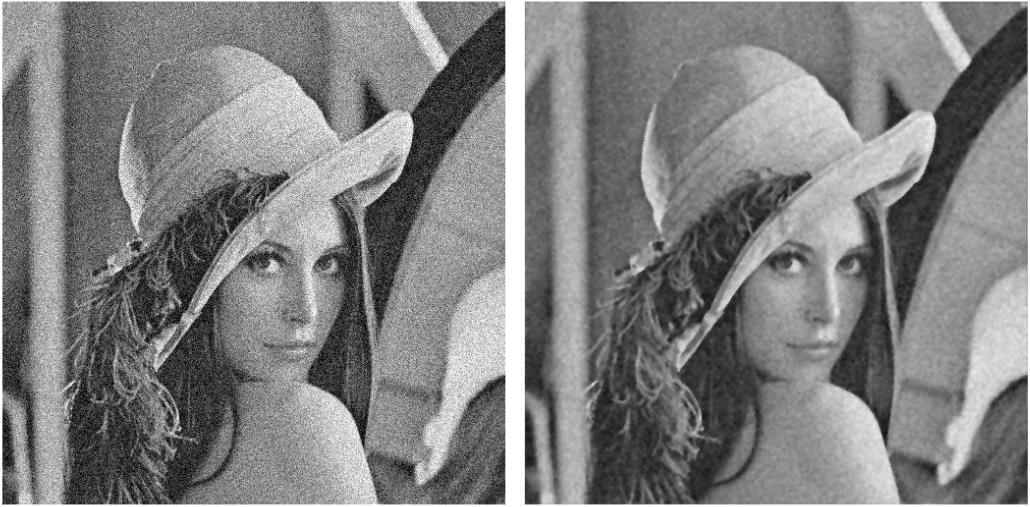
\includegraphics[width=0.6\linewidth] {background/filtering/bilat_filter_eg}
\end{center}
\caption[Example Bilateral Filter]{A bilateral filtering example$\footnotemark$: On the left side a noisy input image on the right its bilateral filtered version.}
\label{fig:bilat_filtering_eg}
\end{figure}
\footnotetext{The shown images have been extracted from: \\ \url{https://www.uni-due.de/mathematik/krommweh/talk_Gemen_Krommweh.pdf}}
The filter replaces the intensity values at each pixel in an image by a weighted average of intensity values from nearby pixels. In our formulation we rely on the Gaussian distributions $G$ for defining the weights. Crucially, the weights depend not only on distances between pixels, but also on the intensity difference. That is why, when iterating through each pixel and adjusting weights to the adjacent pixels accordingly, Sharp edges are preserved. A bilateral filtering example is shown in figure $\ref{fig:bilat_filtering_eg}$.\\ \\
The mathematical definition of this filter is given in equation $\ref{eq:def_bilateral_filter}$. For a given Image $I$ we want to compute its bilateral filtered version by applying the following definition:
\begin{equation}
\begin{aligned}
&\mathcal{F}^{\text{bf}} \{I \} (p) = \frac{1}{W_p} \sum_{q \in \Omega_p} \underbrace{G_{\sigma_s} (\norm{p-q})G_{\sigma_r} (I_p - I_q)}_{w_p} I_q \\	
& \text{where } W_p = \sum_{q \in \Omega_p} G_{\sigma_s} (\norm{p-q})G_{\sigma_r} (I_p - I_q)
\end{aligned}
\label{eq:def_bilateral_filter}
\end{equation}
The set $\Omega_p$ contains all neighboring points within the window that are centered at the image point $p$. The scalar $W_p$ denotes the normalization factor of the filter and $I_p$ represents the image intensity at the pixel position $p$. Please notice that the definition of the bilateral filter is given per pixel, i.e. gives an representation of the filtered pixel intensity. \\ \\
The bilateral filter is controlled by the two parameters $\sigma_s$ and $\sigma_r$. The range variance increases $\sigma_r$, the BF becomes closer to the Gaussian blur filter. In other words, the larger $\sigma_r$ the more weight a pixel with a large intensity deviation gets. However, when increasing the spatial variance $\sigma_s$ results in smoothing larger features, i.e more distant pixels get a larger weight and thus influence the result more. Figure $\ref{fig:bfilter_influence_sigmas}$ demonstrates the influence of these parameters.
\begin{figure}[H]
\begin{center}
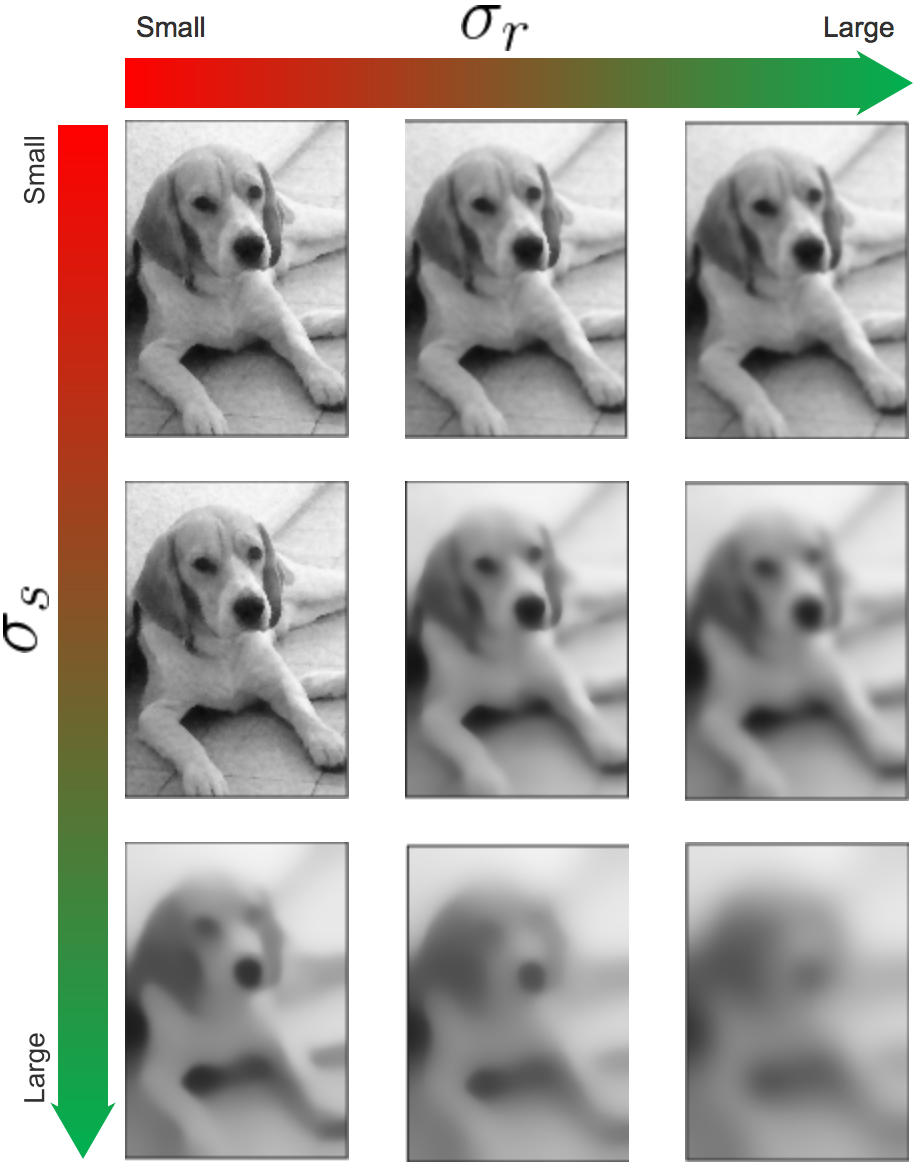
\includegraphics[width=0.6\linewidth] {background/filtering/bilat_filter_sigmas}
\end{center}
\caption[Influence of $\sigma_s$ and $\sigma_r$]{Different filtering results produced by our bilateral filter implementation for varying $\sigma_s$ and $\sigma_r$ values.}
\label{fig:bfilter_influence_sigmas}
\end{figure}

\subsection{Harris Corner Detector}
\label{sec:harris_corner_detector}
Let us consider a grayscale image $I$. We are going to sweep a window $w(x,y)$ (with displacements u in the x direction and v in the right direction) I and will calculate the variation of intensity. Since we are looking for windows with corners, we are looking for windows with a large variation in intensity. Hence, we have to maximize the equation above, specifically the term:
\begin{equation}
	E \left( u, v \right) = \sum_{x,y} w \left( x,y \right) \left[ I(x + u, y + v) - I(x, y) \right]^2
\label{eq:var_intensitiy_def}
\end{equation}
Next, the term $I(x + u, y + v)$ is expressed by the first order taylor series expansion as the follows:
\begin{equation}
	I(x + u, y + v) = I(x,y) + u I_x (x, y) + v I_y (x,y) + \text{h.o.t}
\label{eq:taylor_exp_intensity}
\end{equation}
Next, we put the first order approximation of equation $\ref{eq:taylor_exp_intensity}$ into equation $\ref{eq:var_intensitiy_def}$ to simplify the definition of $E$.
\begin{equation}
\begin{aligned}
E \left( u, v \right) 
&= \sum_{x,y} w \left( x,y \right) \left[ I(x + u, y + v) - I(x, y) \right]^2 \\
&\approx \sum_{x,y} w \left( x,y \right) \left[ I(x,y) + u I_x (x, y) + v I_y (x,y) - I(x, y) \right]^2 \\
&= \sum_{x,y} w \left( x,y \right) \left[ u I_x (x, y) + v I_y (x,y) \right]^2 \\
&= \sum_{x,y} w \left( x,y \right) u^2 I_x^2 + 2 u v I_x I_y v^2 I_y^2 \\
&= \left( u,v \right) \left( \sum_{x,y} w (x,y)
\begin{pmatrix}
I_x^2 & I_x I_y \\
I_x I_y & I_y^2 \\
\end{pmatrix}
\right) \colvec{u}{v}
\end{aligned}
\label{eq:var_intensitiy_developed}
\end{equation}
Let us define the following substitution
\begin{equation}
M = \sum_{x,y} w  (x,y)
\begin{pmatrix}
I_x^2 & I_x I_y \\
I_y^2 & I_x I_y \\
\end{pmatrix}
\label{eq:var_intensity_sub}
\end{equation}
Putting the substitution from equation $\ref{eq:var_intensity_sub}$ into the final form of equation $\ref{eq:var_intensitiy_developed}$ we obtain the final form
\begin{equation}
	E \left( u, v \right) \approx \left( u,v \right) M \colvec{u}{v}
\end{equation}.
A score is calculated for each window, to determine if it can possibly contain a corner:
\begin{equation}
\begin{aligned}
& R = \det(M) - \kappa \left(\text{trace}(M)\right)^2 \\
&\text{where } \det(M) = \lambda_1 \lambda_2 \text{ and } \text{trace}(M) = \lambda_1 + \lambda_2
\end{aligned}
\label{eq:harris_response}
\end{equation}

\section{On Statistics}
\label{sec:on_statistics_bg}

\subsection{Conditional Probability}
Given two events $A$ and $B$ with the probability $P(B) > 0$. The conidtional probability of $A$ given $B$ is defined as
\begin{equation}
	P(A|B) = \frac{P(A \cap B)}{P(B)}
\label{eq:conditional_prob}
\end{equation}
Furthermore, equation $\ref{eq:conditional_prob}$ gives us an alternative interpretation of the probability of an intersection
\begin{equation}
P(A \cap B) = P(A|B)P(B) 	
\end{equation}
The probability that two events happen the same time is the same as the Probability of the event A given B times the probability of event B. Sticking to this definition, we can visualize all possible outcomes of two events happening the same time as shown in figure $\ref{fig:prob_tree_diagram}$.
\begin{figure}[H]
\begin{center}
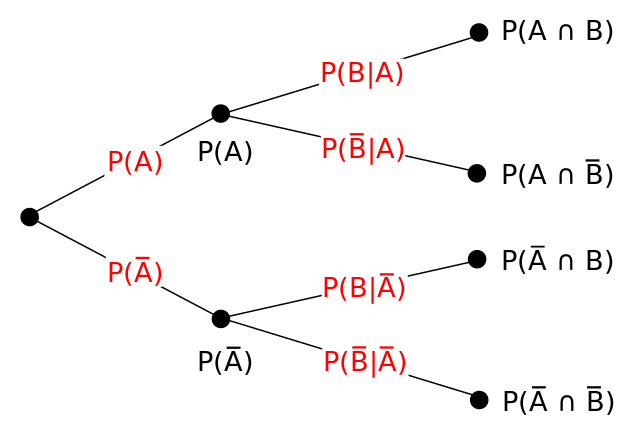
\includegraphics[width=0.45\linewidth] {background/statistics/probability_tree_diagram}
\end{center}
\caption[Probability Tree Diagram]{Tree liked representation$\footnotemark$ of the four possible outcomes for a conditional probability.}
\label{fig:prob_tree_diagram}
\end{figure}
\footnotetext{The visualized graphic has been taken from: \url{https://en.wikipedia.org/wiki/File:Probability_tree_diagram.svg}}



\subsection{Evaluating Binary Classifiers}
In this section we explain the mathematical framework we use in our evaluation.


The purpose of a binary classifier is to classify given elements into two groups according to a specified classification rule. Think about a binary random variable modelling a certain event. The actual observations of the random variable are then either equals true or false. A classification$\footnote{I.e. the produced output after applying the classifier on the given data.}$ of a given dataset yields two numbers: the number of the positives and negatives, which add up to the size of the set. \\ \\
In order to evaluate the quality of binary classifier its prediction is compared against a standard reference method or, if existing, against a ground truth assignment and then cross tabulates the data into a $2 \times 2$ contingency table as shown in figure $\ref{tab:prediction_sensitivity}$. 
\begin{table}[H]
\centering
\begin{tabular}{c|c|c|}
\cline{2-3}
 & \begin{tabular}[c]{@{}l@{}}Prediction\\ Positive\end{tabular} & \begin{tabular}[c]{@{}l@{}}Prediction\\ Negative\end{tabular} \\ \hline
\multicolumn{1}{|l|}{\begin{tabular}[c]{@{}l@{}}Condition\\ Positive\end{tabular}} & \cellcolor[HTML]{34FF34}{\color[HTML]{000000} $\bf{TP}$ } & \cellcolor[HTML]{CB0000} $\bf{FN}$ \\ \hline
\multicolumn{1}{|l|}{\begin{tabular}[c]{@{}l@{}}Condiation\\ Negative\end{tabular}} & \cellcolor[HTML]{CB0000}{\color[HTML]{000000} $\bf{FP}$ } & \cellcolor[HTML]{34FF34} $\bf{TN}$ \\ \hline
\end{tabular}
\caption[Conditional Probability]{The four possible outcomes of a conditional probability}
\label{tab:prediction_sensitivity}
\end{table}
There are four possible outcomes: the classifier prediction, which has either are positive or negative condition, was actually correct or incorrect. \\ \\
Let us consider the following example where we test some people for the presence of a disease. Some of these people have the disease, and the test correctly detects them. These findings are called true positives (\textbf{TP}). Some have the disease, but the test incorrectly claims that they do not have it. These results are called false negatives (\textbf{FN}). Some people do not suffer from the disease and the test classifies correctly as health. These results are called true negatives (\textbf{TN}). And Lastly, some healthy people who are incorrectly classified as infected. These are the so called false positives (\textbf{FP}) results. \\ \\
There are many metrics that can be used to measure the performance of a classifier. In the following a listing of some prominent metrics
%
\begin{itemize}
\item \textbf{Precision}: Tells us what proportion of patients we diagnosed as having the disease actually had that disease. In other words, proportion of TP in the set of positive disease diagnoses. This is given by the rightmost column in the confusion matrix.
\begin{equation}
	\text{precision} = \frac{\text{TP}}{\text{TP} + \text{FP}}
\label{eq:def_precision}
\end{equation}
\item \textbf{Recall}: Tells us what proportion of people that actually had the disease were diagnosed by the test as having the disease. In other words, proportion of TP in the set of true disease states. This is given by the bottom row in the confusion matrix.
\begin{equation}
	\text{recall} = \frac{\text{TP}}{\text{TP} + \text{FN}}
\label{eq:def_recall}
\end{equation}
\end{itemize}
A visualization of these measures is given in figure $\ref{fig:eval_concept_recall_precc}$.
\begin{figure}[H]
\begin{center}
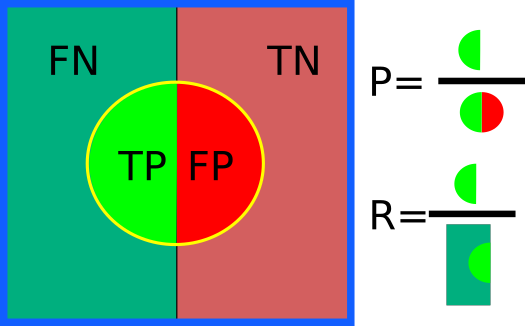
\includegraphics[width=0.6\linewidth] {evaluation/prec_recall}
\end{center}
\caption[Concept Recall and Precision]{This figure illustrates graphically the concept of Recall (\textbf{R}) and Precision (\textbf{P}). When estimating the sampling of a binary random variable, there are basically four possible outcomes: The we predicted it being true and it is true (\textbf{TP}), we predicted it true but it is false (\textbf{FP}), we predicted it false and it was actually negative (\textbf{FN}) or we predicted it to be true but it was actually false (\textbf{TN}). }
\label{fig:eval_concept_recall_precc}
\end{figure}
An alternative measure is the $F_1$ score. This measure is often used in determining the performance of classification tasks in machine learning. To compute its score, this measure takes into account both, the precision and the recall of the test. The exact definition of the F1 measure is given in equation $\ref{eq:f1_score}$.
\begin{equation}
F_1 = 2 \left( \frac{\text{precision} \times \text{recall}}{\text{precision} +\text{recall}} \right)
\label{eq:f1_score}
\end{equation}  
The F1 score can be interpreted as a normalized weighted average of the precision and recall measures. The best possible F1 score is equals 1 and its worst value is 0.

\section{Camera Model}
\subsection{Pinhole Camera}
A camera projects a 3d scene in a 2d image. A simple mathematical model to describe such a mapping from the 3d scene space to the 2d image space is the pinhole camera model. This model is conceptually illustrated in figure $\ref{fig:pinhole_camera_model}$.
\begin{figure}[H]
\begin{center}
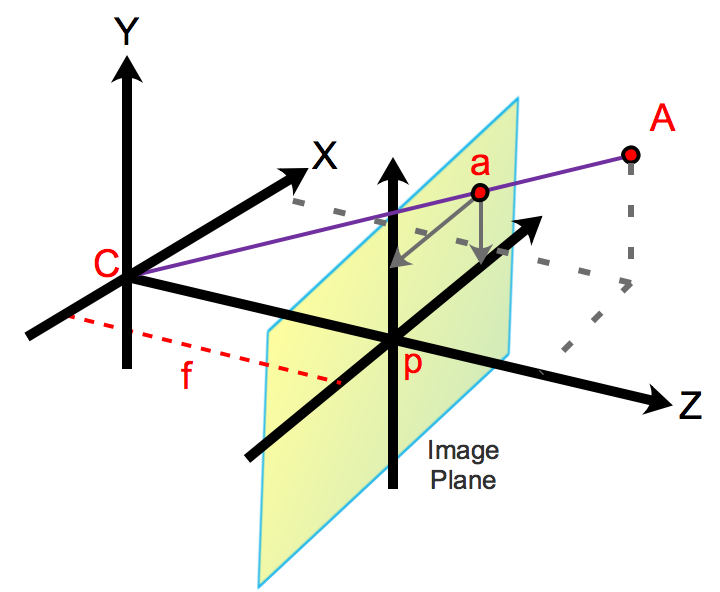
\includegraphics[width=0.8\linewidth] {background/camera_model/pinhole_camera}
\end{center}
\caption[Pinhole Camera Model]{Visualizing the pinhole camera model. The camera center $C$ represents an infinitely small aperture hole and assumed to be located at $(0,0,0)$, $f$ is the focal length in pixel units, $p$ is the principal point in images coordinates, $\textbf{A} = (X, Y, Z)$ a 3d point in the scene and $\textbf{a} = (f \frac{X}{Z}, f \frac{Y}{Z})$ its projected pixel version mapped onto the image plane.}
\label{fig:pinhole_camera_model}
\end{figure}
The aperture is an infinitely small hole and there is no lens used to focus light. Therefore, lens distorting or depth of field effects are ignored. The intersection point where all rays meet is the center of the perspective projection and usually referred by \textit{camera center}. The principal axis is formed by the line perpendicular to the image plane, which passes though the camera center. Its intersection point with the image plane is called principal point. The distance between the camera center and the principal point is the so called focal length.

\subsection{Camera Parameters}
\paragraph{Intrinsic Parameters} Let $\textbf{X} = (X,Y,Z,1)^T$ denote a point in a 3D scene and $\textbf{x} = (x,y,1)^T$ its projected version in the image plane. Both points are written in their homogeneous form. The mapping from a scene point to the image plane is defined as
\begin{equation}
\textbf{x} = 
\begin{pmatrix}
f & s & p_x & 0 \\
0 & f & p_y & 0 \\
0 & 0 & 1 & 0
\end{pmatrix}
\textbf{X}
\end{equation}
where $f$ denotes the focal length and $p = (p_x, p_y)^T$ the offset to the origin in image coordinates with respect to the principal point. In modern cameras, the skew $s$ is usually equals zero. The parameters $f$, $p_x$, $p_y$ and $s$ are called \textit{intrinsic camera parameters}. Notice, that $\textbf{X}$ is expressed in terms of camera coordinates and similarly, $\textbf{x}$ in pixel coordinates.

\paragraph{Extrinsic Parameters} In general, a camera is not located at the origin of the world coordinate system and can have an arbitrary orientation. Let $\textbf{X}_w$ denote a point, living in an arbitrary camera coordinate system. To express this point in the regular camera coordinate system, we have to apply a certain transformation. In a rigid object model, the points $\textbf{X}$ and $\textbf{X}_w$ can be transformed to one another by applying a linear transformation that consists of a rotational matrix $R$ and a translation $t$. The actual mapping is defined as
\begin{equation}
	X = \left[ R | t \right] X_w
\end{equation}
The parameters $t$ and $R$ are called \textit{extrinsic camera parameters}.


%%% CLEAN UP
\chapter{Experiment Statistics}
\label{sec:appendix_varying_lambda}

\begin{table}[H]
\centering
\begin{tabular}{|c|c|c|c|}
\hline
\multicolumn{4}{|c|}{PD Varying $\lambda$ on PD cars}                        \\ \hline
$\lambda$ & \textbf{Precision} & \textbf{Recall} & \textbf{F1 Score} \\ \hline
5 & 11.68 & 10.73\% & 11.18\%  \\ \hline
1 & 15.68 & 11.51\% & 13.28\%  \\ \hline
0.1 & 34.05 & 30.08\% & 31.94\%  \\ \hline
\textbf{0.01} & \textbf{46.37} & \textbf{52.94}\% & \textbf{49.44}\%  \\ \hline
0.001 & 43.00 & 45.67\% & 44.29\%  \\ \hline
0.0001 & 25.11 & 25.78\% & 25.44\%  \\ \hline
\end{tabular}
\caption[Cars Varying $\lambda$]{My caption}
\label{tab:cars_varying_lambas}
\end{table}



\chapter{Experiments}
In this section we list the results of a series of experiments we performed running our pipeline on the presented dataset from section $\ref{sec:datasets}$ on page $\pageref{sec:datasets}$. The results are evaluated according the previously explained measures from section $\ref{sec:methodology}$ on page $\pageref{sec:methodology}$. \\ \\
For performing our experiments we used MacBook Pro. The hardware specifications of this machine are listed in table $\ref{tab:used_hardware_specs}$. 
\begin{table}[H]
\centering
\begin{tabular}{|l|c|}
\hline
\multicolumn{2}{|c|}{\textbf{Hardware Specifications}} \\ \hline
\textbf{CPU} & 2.5 GHz Intel Core i7 \\ \hline
\textbf{Threads} & 8 \\ \hline
\textbf{MEMORY} & 16 GB 1600 MHz DDR3 \\ \hline
\textbf{GPU} & Intel Iris Pro 1536 MB \\ \hline
\end{tabular}
\caption{A listing of the hardware specifications of the used machine to produce the results.}
\label{tab:used_hardware_specs}
\end{table}

\subsection{Varying Pipeline Combinations for LDOF flows}
%START EXPERIMENT SETUP
chairs dataset
use only LDOF flows
affinity generation / segmentation techniques combinations
pipeline modes: PD SC, PD MC, PED SC, PED MC, SD KL, SED KL.
solve for 10 fixed clusters and evaluate the resulting segments on two different kinds of masks: real and simple case.
Which setting is the best?

moreover, evaluate the quality of LDOF SED KL segmentation by altering the number of clusters we want to solve for.
% END EXPERIMENT SETUP


The \textit{Bonn Chairs} dataset is a video sequence consisting of 58 frames. It shows a room containing two chairs and a man. The man is moving the and rotating the right chair. Also, the camera is moving. See figure $\ref{fig:eval_bonn_chairs_frames}$ to get a better understanding of the whole scene.
\begin{figure}[H]
\begin{center}
\subfigure[Frame 1]{
   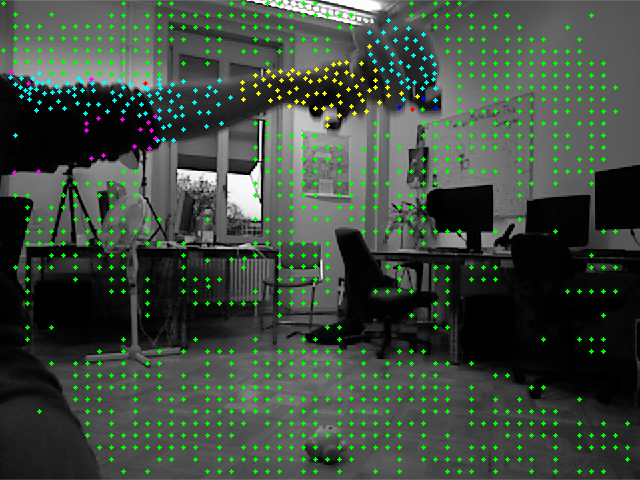
\includegraphics[width=0.31\linewidth] {evaluation/bonn_chairs_frames/1}
   \label{fig:eval_bonn_chairs_frames_a}
}
\subfigure[Frame 12]{
   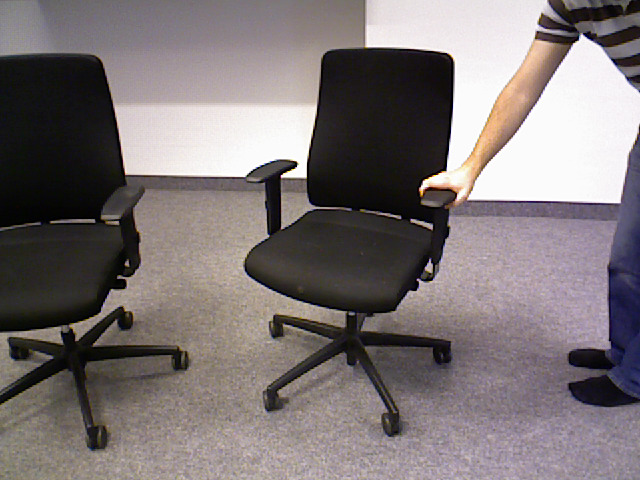
\includegraphics[width=0.31\linewidth] {evaluation/bonn_chairs_frames/12}
   \label{fig:eval_bonn_chairs_frames_b}
}
\subfigure[Frame 24]{
   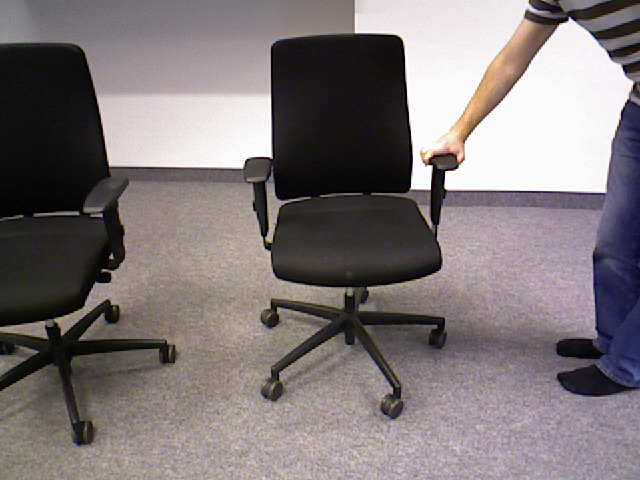
\includegraphics[width=0.31\linewidth] {evaluation/bonn_chairs_frames/24}
   \label{fig:eval_bonn_chairs_frames_c}
}
~
\subfigure[Frame 35]{
   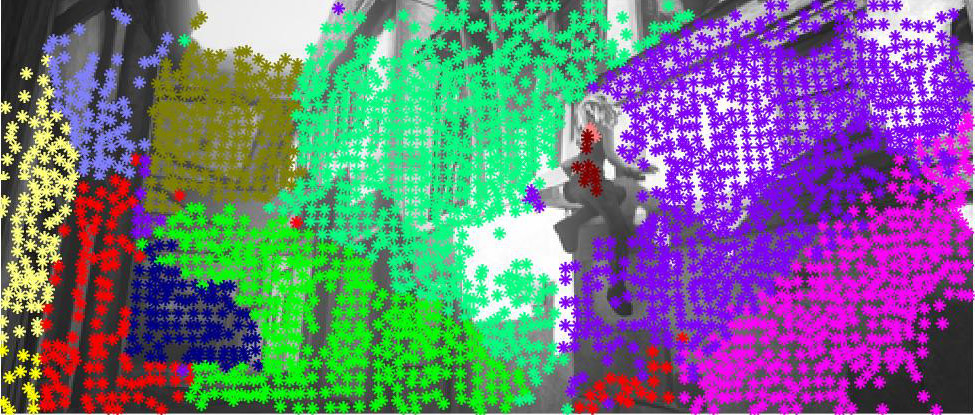
\includegraphics[width=0.31\linewidth] {evaluation/bonn_chairs_frames/35}
   \label{fig:eval_bonn_chairs_frames_a}
}
\subfigure[Frame 47]{
   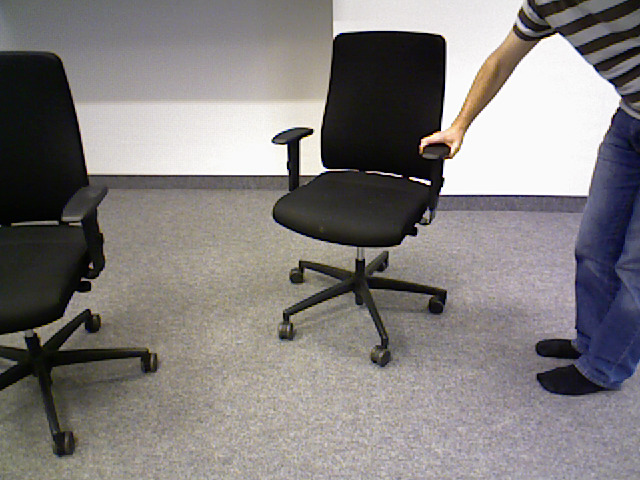
\includegraphics[width=0.31\linewidth] {evaluation/bonn_chairs_frames/47}
   \label{fig:eval_bonn_chairs_frames_b}
}
\subfigure[Frame 58]{
   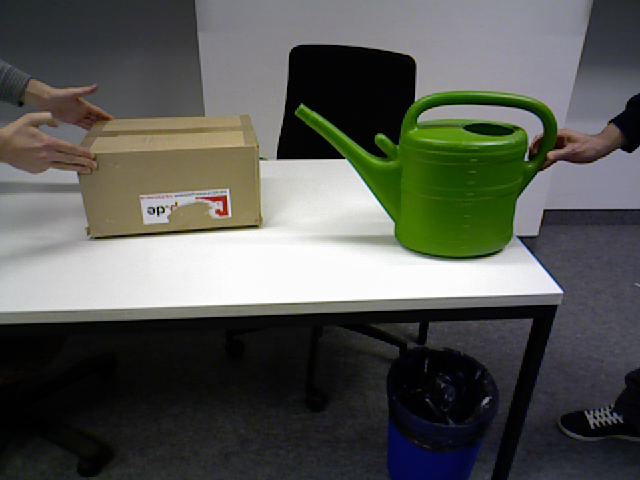
\includegraphics[width=0.31\linewidth] {evaluation/bonn_chairs_frames/58}
   \label{fig:eval_bonn_chairs_frames_c}
}
\end{center}
\caption[Bonn Chairs Dataset]{Listing of 6 ascending frames of the our Bonn Chairs dataset. In this dataset we have a scene in which there are 2 chairs and a man in a room. The man is moving and rotating the right chair. The same time, also the camera is slightly moving around.}
\label{fig:eval_bonn_chairs_frames}
\end{figure}
This dataset contains depth images as well as camera calibration data. The depth-and color camera are already aligned. \\ \\
For the following experiment we only use LDOF flows. Moreover, we fix the number of clusters we want to solve for and set it equal to six segments. In our pipeline we run all valid cross combinations between our affinity computation methods, such as PD, PED, SD and SED and the segmentation methods SC, MC and KL. The resulting segmentations are shown in figure $\ref{fig:eval_bonn_chairs_raw_segmentations}$.
% foo

% new gt 30
\begin{figure}[H]
\begin{center}
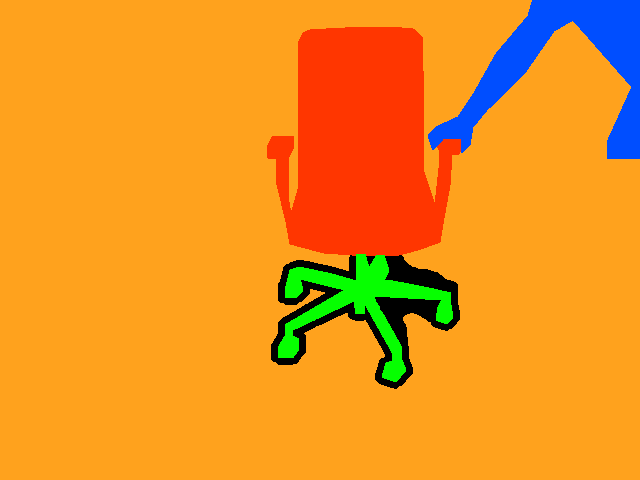
\includegraphics[width=0.48\linewidth] {evaluation/bonn_chairs_c_10_segmentations_f_30/30_amb}
\end{center}
\caption[Bonn Chairs GT Frame 30]{Ground truth frame No. 30 of the Bonn Chairs dataset.}
\label{fig:eval_bonn_chairs_gt_30}
\end{figure}
% end new gt 30

% new raw segmentations frame 30
\begin{figure}[H]
\begin{center}
\subfigure[LDOF PD SC]{
   \includegraphics[width=0.48\linewidth] {evaluation/bonn_chairs_c_10_segmentations_f_30/ldof_pd_sc}
   \label{fig:eval_bonn_chairs_raw_segmentations_frame_30_a}
}
\subfigure[LDOF PD MC]{
   \includegraphics[width=0.48\linewidth] {evaluation/bonn_chairs_c_10_segmentations_f_30/ldof_pd_mc}
   \label{fig:eval_bonn_chairs_raw_segmentations_frame_30_b}
}
~
\subfigure[LDOF PED SC]{
   \includegraphics[width=0.48\linewidth] {evaluation/bonn_chairs_c_10_segmentations_f_30/ldof_ped_sc}
   \label{fig:eval_bonn_chairs_raw_segmentations_frame_30_c}
}
\subfigure[LDOF PED MC]{
   \includegraphics[width=0.48\linewidth] {evaluation/bonn_chairs_c_10_segmentations_f_30/ldof_ped_mc}
   \label{fig:eval_bonn_chairs_raw_segmentations_frame_30_d}
}
~
\subfigure[LDOF SD KL]{
   \includegraphics[width=0.48\linewidth] {evaluation/bonn_chairs_c_10_segmentations_f_30/ldof_sd_kl}
   \label{fig:eval_bonn_chairs_raw_segmentations_frame_30_e}
}
\subfigure[LDOF SED KL]{
   \includegraphics[width=0.48\linewidth] {evaluation/bonn_chairs_c_10_segmentations_f_30/ldof_sed_kl}
   \label{fig:eval_bonn_chairs_raw_segmentations_frame_30_f}
}
\end{center}
\caption[Bonn Chairs Segmentations Frame 30]{Segmentations produced by our pipeline when running the Bonn Chairs dataset, using 10 clusters.}
\label{fig:eval_bonn_chairs_raw_segmentations_frame_30}
\end{figure}
% end raw segmentations frame 30


% TODO list qualitative observations here, old version is below:
%Ideally, a segmentation should have a separate mask for the man's arm, the lower parts (the seat and the star base) of the office chair and its backrest, as well as one for the background.
%
%At a first glance, are methods were performing rather well, being capable of detecting all these expected masks. However, there is still a difference in the their result's quality. Especially around the region of the men's arm, we observe a difference of quality when comparing methods that make use of depth information with those not making use of any depth. Non-depth using methods tend to assign points to the arm's cluster which should belong to the background. This could however be due to the fact that such points are spatially close to the arm and thus exhibit a large affinity value to the trajectories within the arm region. \\ \\
%Interestingly, the SD KL method was oversegmenting the chair's seat into two clusters. One possible explanation for this could be, that we were using a too large probability value when using six clusters. \\ \\
%Some methods seem to have trouble in correctly segmenting the chair's arm lean, especially all MC clustering methods seem to have issues in correctly assigning this region. \\ \\
%Last, please notice that we used many more cluster for the SED KL method, since it performed very poor when using six clusters. The actual result when using 6 only six clusters is shown in figure $\ref{fig:bonn_chairs_sed_varyingclusters}$. The reason why we legitimate ourself to use this 10 cluster result is stated below.
%
%STATE SOME QUALITATIVE OBSERVATIONS HERE. \\ \\
%
%For measuring the quantitative performance of the resulting segmentations we compare their merged cluster versions, which are shown in figure $\ref{fig:eval_bonn_chairs}$, with the ground truth mask as depcited in figure $\ref{fig:eval_bonn_chairs_gt_20}$.


% new bonn chairs fig
\begin{figure}[H]
\begin{center}
\subfigure[LDOF PD SC]{
   \includegraphics[width=0.48\linewidth] {evaluation/bonn_chairs_c_10/ldof_pd_sc}
   \label{fig:bonn_chairs_c_10_b}
}
\subfigure[LDOF PD MC]{
   \includegraphics[width=0.48\linewidth] {evaluation/bonn_chairs_c_10/ldof_pd_mc}
   \label{fig:bonn_chairs_c_10_c}
}
~
\subfigure[LDOF PED SC]{
   \includegraphics[width=0.48\linewidth] {evaluation/bonn_chairs_c_10/ldof_ped_sc}
   \label{fig:bonn_chairs_c_10_d}
}
\subfigure[LDOF PED MC]{
   \includegraphics[width=0.48\linewidth] {evaluation/bonn_chairs_c_10/ldof_ped_mc}
   \label{fig:bonn_chairs_c_10_e}
}
~
\subfigure[LDOF SD KL]{
   \includegraphics[width=0.48\linewidth] {evaluation/bonn_chairs_c_10/ldof_sd_kl}
   \label{fig:bonn_chairs_c_10_d}
}
\subfigure[LDOF SED KL]{
   \includegraphics[width=0.48\linewidth] {evaluation/bonn_chairs_c_10/ldof_sed_kl}
   \label{fig:bonn_chairs_c_10_e}
}
\end{center}
\caption[Merged Segments Bonn Chairs]{Final, merged segmentation results of frame 30 when running our pipeline on the bonn dataset. The quantitive measures of these segmentations are listed in table $\ref{tab:eval_bonn_chairs}$.}
\label{fig:eval_bonn_chairs_c_10}
\end{figure}
% end new bonn chairs fig

% new bc table
\begin{table}[H]
\centering
\begin{tabular}{|l|l|l|l|l|l|}
\hline
\multicolumn{6}{|c|}{Comparison bonn chairs dataset using 10 clusters}                        \\ \hline
\textbf{Method} & \textbf{Density} & \textbf{Precision} & \textbf{Recall} & \textbf{F1 Score} & \textbf{Fragmentation} \\ \hline
LDOF PD SC & 0.41/0.43 & 49.98/47.48 \%   & 61.88/61.88 \%     & 55.29/53.73 \%  & x \% \\ \hline
LDOF PD MC & 0.41/0.43 & 45.30/42.46 \%   & 66.10/66.10 \%     & 53.75/51.70 \%  & x \%   \\ \hline
LDOF PED SC & 0.34/0.35& 59.54/56.86 \%   & 47.35/47.35 \%     & 52.75/51.67 \%  & x \%   \\ \hline
LDOF PED MC & 0.34/0.35 & 59.30/56.68 \%   & 50.56/50.56 \%     & 54.58/53.44 \%  & x \%   \\ \hline              
LDOF SD KL & 0.41/0.43 & 48.46/46.34 \%   & 63.44/63.44 \%     & 54.95/53.56 \%  & x \%   \\ \hline
LDOF SED KL & 0.34/0.36 & 91.34/64.42 \%   & 81.60/64.63 \%     & 86.20/64.52 \%    & x \%  \\ \hline
\end{tabular}
\caption[Bonn Chairs Merged 10 Clusters]{}
\label{tab:eval_bonn_chairs_c_10}
\end{table}
% end new bc table




% TODO: weg damit mit easy mask

%TODO mention some facts about the qualitative properties of the segmentations.

\begin{figure}[H]
\begin{center}
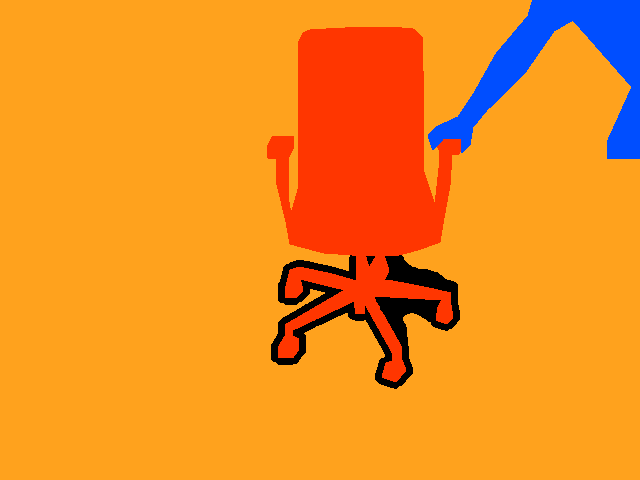
\includegraphics[width=0.48\linewidth] {evaluation/bonn_chairs_c_10_segmentations_f_30/30_easy_amb}
\end{center}
\caption[Bonn Chairs Simple GT Frame 30]{Simplified ground truth frame No. 30 of the Bonn Chairs dataset.}
\label{fig:eval_bonn_chairs_simple_gt_30}
\end{figure}

% Make table including statistics
\begin{figure}[H]
\begin{center}
\subfigure[LDOF PD SC]{
   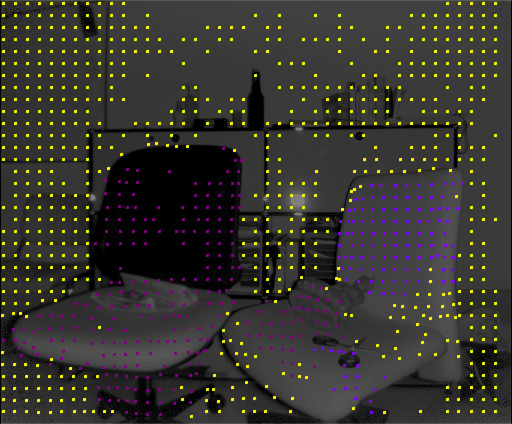
\includegraphics[width=0.48\linewidth] {evaluation/bonn_chairs_c_10_merged_simple/pd_sc}
   \label{fig:bonn_chairs_c_10_simple_b}
}
\subfigure[LDOF PD MC]{
   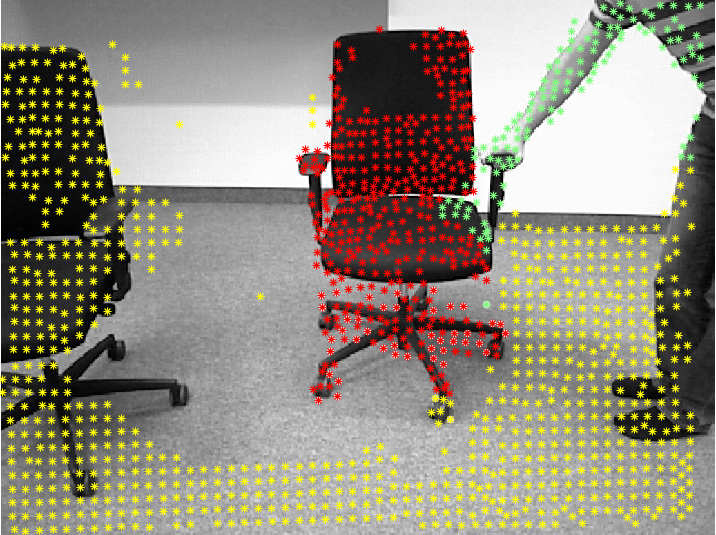
\includegraphics[width=0.48\linewidth] {evaluation/bonn_chairs_c_10_merged_simple/pd_mc}
   \label{fig:bonn_chairs_c_10_simple_c}
}
~
\subfigure[LDOF PED SC]{
   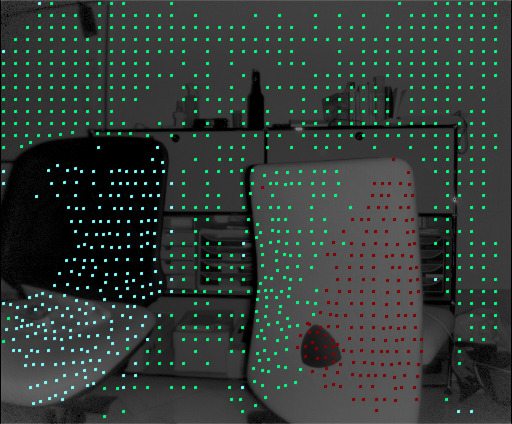
\includegraphics[width=0.48\linewidth] {evaluation/bonn_chairs_c_10_merged_simple/ped_sc}
   \label{fig:bonn_chairs_c_10_simple_d}
}
\subfigure[LDOF PED MC]{
   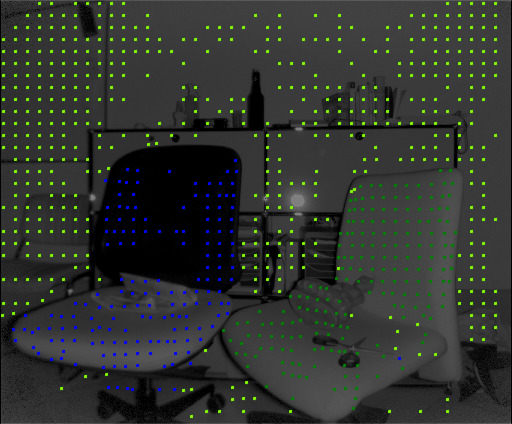
\includegraphics[width=0.48\linewidth] {evaluation/bonn_chairs_c_10_merged_simple/ped_mc}
   \label{fig:bonn_chairs_c_10_simple_e}
}
~
\subfigure[LDOF SD KL]{
   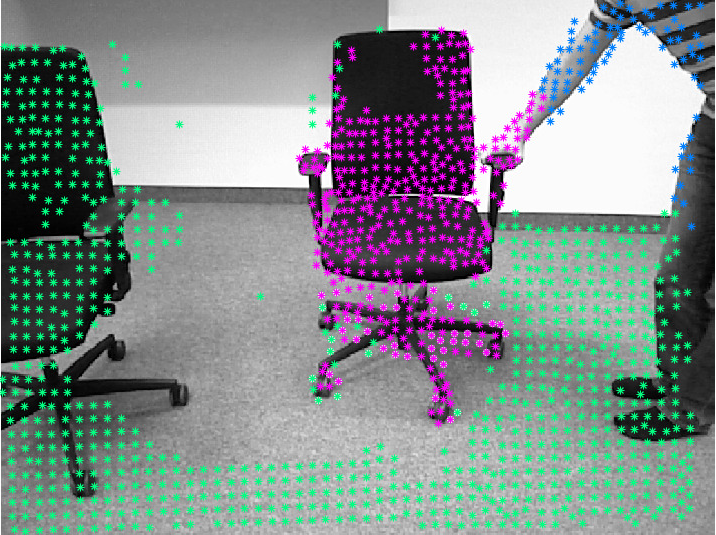
\includegraphics[width=0.48\linewidth] {evaluation/bonn_chairs_c_10_merged_simple/sd_kl}
   \label{fig:bonn_chairs_c_10_simple_d}
}
\subfigure[LDOF SED KL]{
   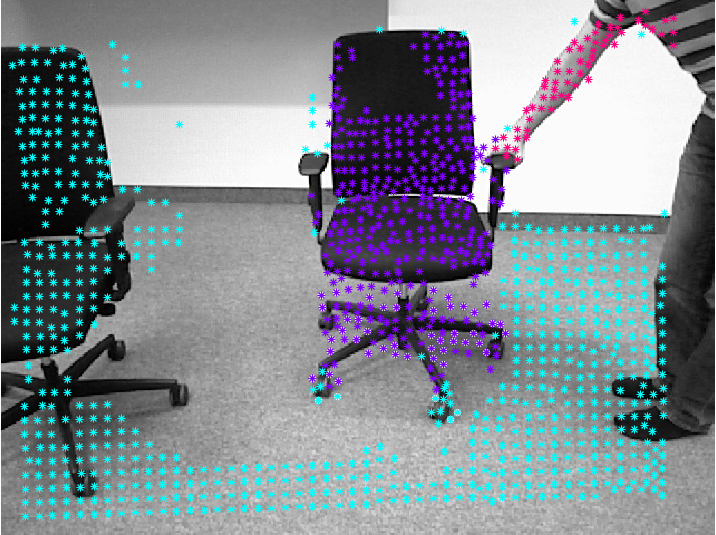
\includegraphics[width=0.48\linewidth] {evaluation/bonn_chairs_c_10_merged_simple/sed_kl}
   \label{fig:bonn_chairs_c_10_simple_e}
}
\end{center}
\caption[Simple Merged Segments Bonn Chairs]{Final, merged segmentation results of frame 30 when running our pipeline on the bonn dataset. The quantitive measures of these segmentations are listed in table $\ref{tab:eval_bonn_chairs}$.}
\label{fig:eval_bonn_chairs_c_10_simple}
\end{figure}

% Make merged table
\begin{table}[H]
\centering
\begin{tabular}{|l|l|l|l|l|}
\hline
\multicolumn{5}{|c|}{Comparison bonn chairs dataset using 10 clusters using the simple mask}                        \\ \hline
\textbf{Method} & \textbf{Density} & \textbf{Precision} & \textbf{Recall} & \textbf{F1 Score} \\ \hline
LDOF PD SC & 0.41113 & 82.4671 \%   & 90.7807 \%     & 86.4244 \% \\ \hline
LDOF PD MC & 0.41113 & 75.8905 \%   & 95.3212 \%     & 84.5033 \%  \\ \hline
LDOF PED SC & 0.33594 & 97.2414 \%   & 69.1012 \%     & 80.791 \%  \\ \hline
LDOF PED MC & 0.33594 & 96.6997 \%   & 73.6677 \%     & 83.6268 \%  \\ \hline              
LDOF SD KL & 0.41146 & 79.7901 \%   & 91.2061 \%     & 85.117 \%    \\ \hline
LDOF SED KL & 0.34147 & 95.9657 \%   & 86.5871 \%     & 91.0355 \%  \\ \hline
\end{tabular}
\caption[Bonn Chairs Merged 10 Clusters]{}
\label{tab:eval_bonn_chairs_c_10_simple}
\end{table}


\subsection{Varying Cluster Count on SED KL}
% foo
Please notice that the performance of the $\textit{LDOF\_SED\_KL}$ is very poor for this cluster assignment. The reason for this is because this method was not well parameterized, resulting in a large oversegmentation. However, since this optimal parameter assignment exists, but was not found, we further investigated the performance by performing two additional experiments. The SED method was run, once using 9 clusters (indicated by SED* KL), and once again using 10 clusters (SED** KL). As we can see, the method LDOF SED** KL is superior compared to every other method run on this dataset. The actual segmentation results of the different SED methods are shown in figure $\ref{fig:bonn_chairs_sed_varyingclusters}$.
\begin{figure}[H]
\begin{center}
\subfigure[2 Clusters]{
   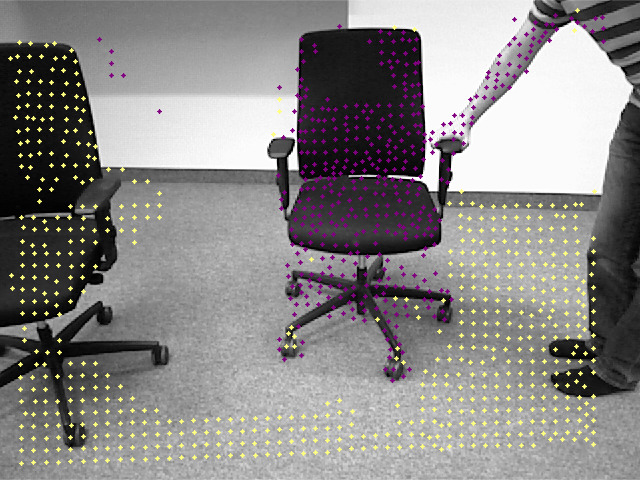
\includegraphics[width=0.31\linewidth] {evaluation/bonn_chairs_ldof_varying_c_sed/f_30_c_2}
   \label{fig:bonn_chairs_sed_varyingclusters_a}
}
\subfigure[3 Clusters]{
   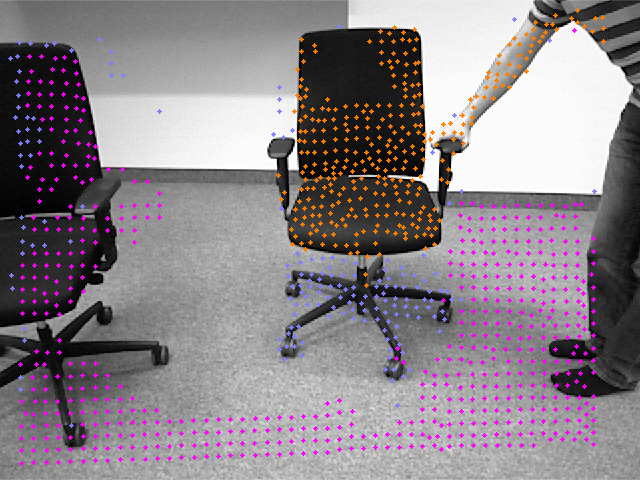
\includegraphics[width=0.31\linewidth] {evaluation/bonn_chairs_ldof_varying_c_sed/f_30_c_3}
   \label{fig:bonn_chairs_sed_varyingclusters_b}
}
\subfigure[4 Clusters]{
   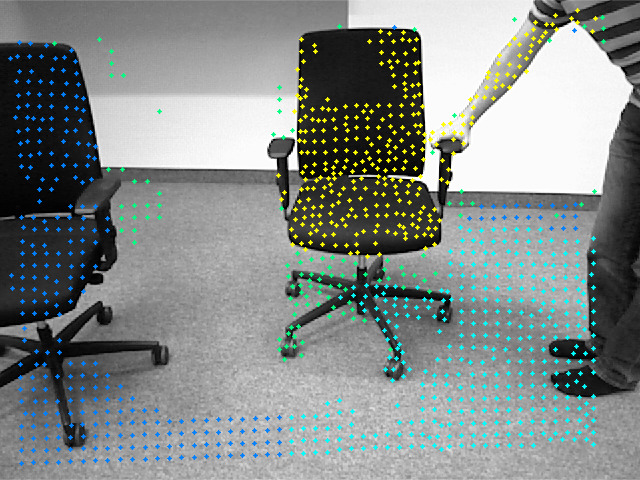
\includegraphics[width=0.31\linewidth] {evaluation/bonn_chairs_ldof_varying_c_sed/f_30_c_4}
   \label{fig:bonn_chairs_sed_varyingclusters_c}
}
~
\subfigure[5 Clusters]{
   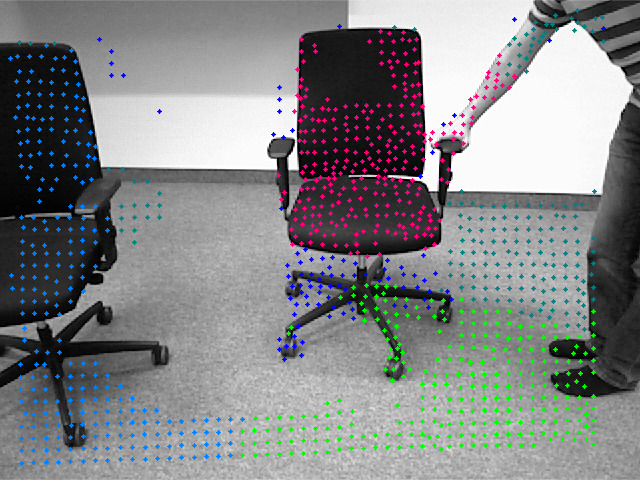
\includegraphics[width=0.31\linewidth] {evaluation/bonn_chairs_ldof_varying_c_sed/f_30_c_5}
   \label{fig:bonn_chairs_sed_varyingclusters_a}
}
\subfigure[6 Clusters]{
   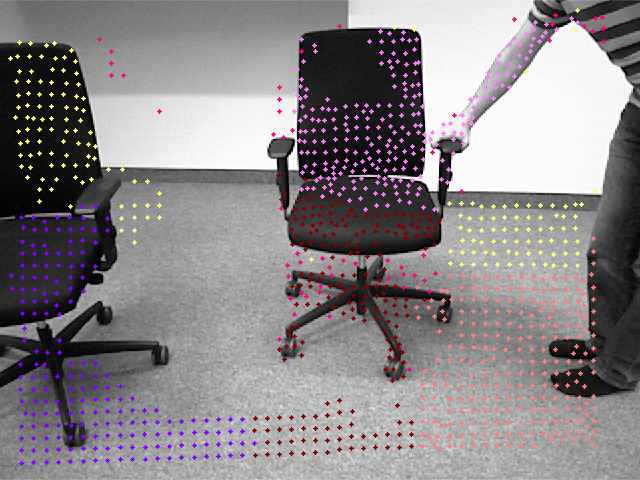
\includegraphics[width=0.31\linewidth] {evaluation/bonn_chairs_ldof_varying_c_sed/f_30_c_6}
   \label{fig:bonn_chairs_sed_varyingclusters_b}
}
\subfigure[7 Clusters]{
   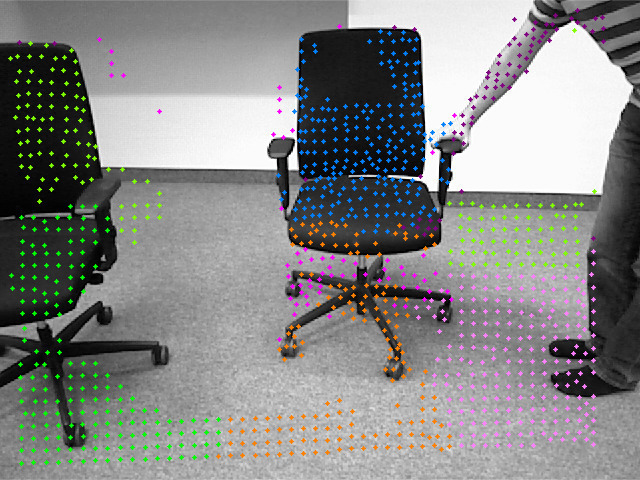
\includegraphics[width=0.31\linewidth] {evaluation/bonn_chairs_ldof_varying_c_sed/f_30_c_7}
   \label{fig:bonn_chairs_sed_varyingclusters_c}
}
~
\subfigure[8 Clusters]{
   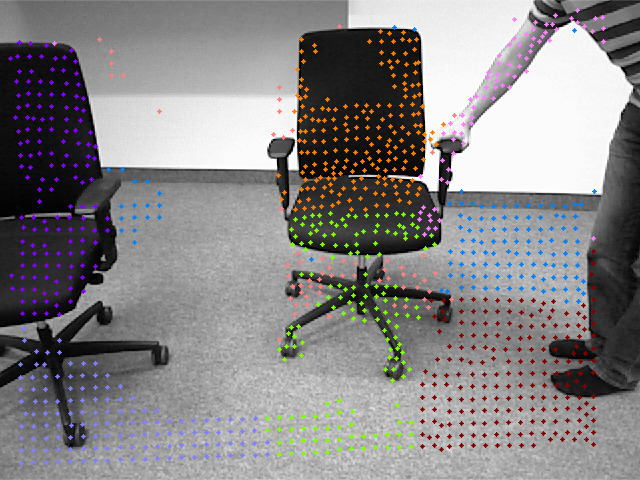
\includegraphics[width=0.31\linewidth] {evaluation/bonn_chairs_ldof_varying_c_sed/f_30_c_8}
   \label{fig:bonn_chairs_sed_varyingclusters_a}
}
\subfigure[9 Clusters]{
   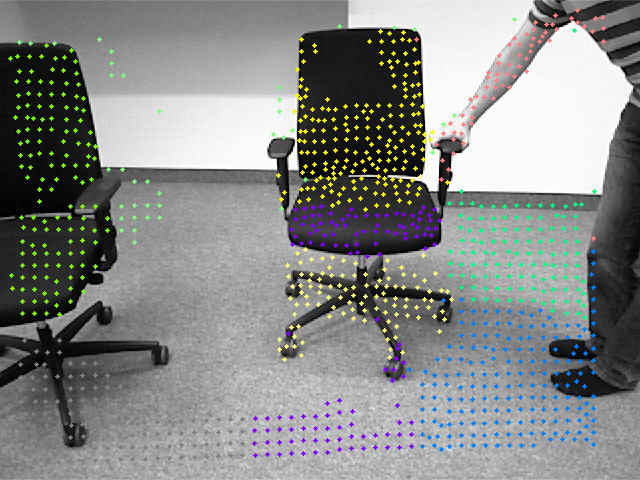
\includegraphics[width=0.31\linewidth] {evaluation/bonn_chairs_ldof_varying_c_sed/f_30_c_9}
   \label{fig:bonn_chairs_sed_varyingclusters_b}
}
\subfigure[10 Clusters]{
   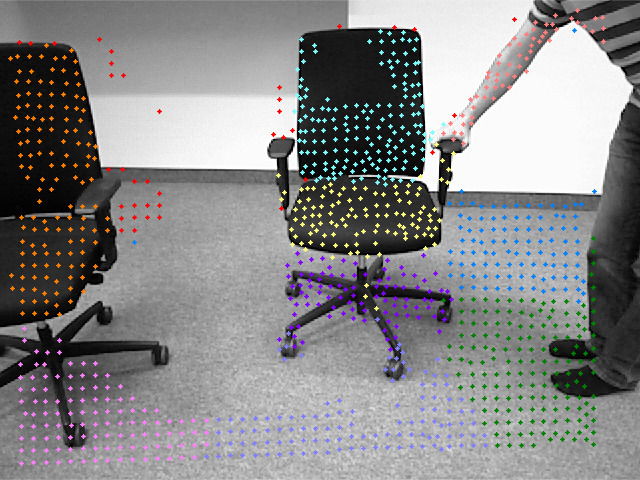
\includegraphics[width=0.31\linewidth] {evaluation/bonn_chairs_ldof_varying_c_sed/f_30_c_10}
   \label{fig:bonn_chairs_sed_varyingclusters_c}
}
\end{center}
\caption[Bonn Chairs SED Segmentations for Varying Cluster Count]{A visualization of the real segmentations when running \textit{SED KL} on the \textit{bonn chairs} dataset.}
\label{fig:bonn_chairs_sed_varyingclusters}
\end{figure}


\begin{table}[H]
\centering
\begin{tabular}{|c|c|c|c|c|}
\hline
\multicolumn{5}{|c|}{Bonn Chairs LDOF SED Varying Clusters}                        \\ \hline
\textbf{Clusters} & \textbf{Density} & \textbf{Precision} & \textbf{Recall} & \textbf{F1 Score} \\ \hline
2 & 0.34 & 22.08\%   & 33.21\%     & 26.53\%  \\ \hline
3 & 0.34 & 26.41\%   & 33.21\%     & 29.42\%  \\ \hline
4 & 0.34 & 26.95\%   & 33.08\%     & 29.70\%  \\ \hline
5 & 0.34 & 29.54\%   & 32.96\%     & 31.16\%  \\ \hline
6 & 0.34 & 20.88\%   & 32.96\%     & 25.57\%  \\ \hline
7 & 0.34 & 56.53\%   & 49.51\%     & 52.79\%  \\ \hline
8 & 0.34 & 48.55\%   & 65.27\%     & 55.68\%  \\ \hline
9 & 0.34 & 82.46\%   & 93.58\%     & 87.67\%  \\ \hline              
10 & 0.34 & 95.97\%   & 86.59\%     & 91.04\%  \\ \hline
\end{tabular}
\caption[Bonn Chairs SED Varying Clusters]{foobar}
\label{tab:bonn_chairs_ldof_sed_c_6_9_10_eval}
\end{table}
%bar

%ldof pd sc
\begin{table}[H]
\centering
\begin{tabular}{|c|c|c|c|c|}
\hline
\multicolumn{5}{|c|}{Bonn Chairs LDOF PD SC Varying Clusters}                        \\ \hline
\textbf{Clusters} & \textbf{Density} & \textbf{Precision} & \textbf{Recall} & \textbf{F1 Score} \\ \hline
2 & 0.41 & 0.0\%   & 0.0\%     & 0.0\%  \\ \hline
3 & 0.41 & 18.30\%   & 9.76\%     & 12.73\%  \\ \hline
4 & 0.41 & 25.30\%   & 28.00\%     & 26.58\%  \\ \hline
5 & 0.41 & 23.46\%   & 19.86\%     & 21.51\%  \\ \hline
6 & 0.41 & 40.28\%   & 30.44\%     & 34.68\%  \\ \hline
7 & 0.41 & 49.88\%   & 66.01\%     & 56.83\%  \\ \hline
8 & 0.41 & 49.81\%   & 58.35\%     & 53.75\%  \\ \hline
9 & 0.41 & 49.86\%   & 65.38\%     & 56.57\%  \\ \hline              
10 & 0.41 & 49.98\%   & 61.88\%     & 55.29\%  \\ \hline
\end{tabular}
\caption[Bonn Chairs PD SC Varying Clusters]{foobar}
\label{tab:bonn_chairs_ldof_sed_c_6_9_10_eval_pd_sc}
\end{table}
% end

%sdf
\begin{table}[H]
\centering
\begin{tabular}{|c|c|c|c|c|}
\hline
\multicolumn{5}{|c|}{Bonn Chairs LDOF PED MC Varying Clusters}                        \\ \hline
\textbf{Clusters} & \textbf{Density} & \textbf{Precision} & \textbf{Recall} & \textbf{F1 Score} \\ \hline
2 & 0.34 & 33.33\%   & 16.92\%     & 22.45\%  \\ \hline
3 & 0.34 & 26.55\%   & 23.23\%     & 24.78\%  \\ \hline
4 & 0.34 & 26.17\%   & 29.55\%     & 27.76\%  \\ \hline
5 & 0.34 & 26.20\%   & 24.12\%     & 25.12\%  \\ \hline
6 & 0.34 & 58.94\%   & 54.44\%     & 56.60\%  \\ \hline
7 & 0.34 & 58.97\%   & 46.03\%     & 51.70\%  \\ \hline
8 & 0.34 & 58.47\%   & 43.61\%     & 49.96\%  \\ \hline
9 & 0.34 & 59.39\%   & 55.24\%     & 57.24\%  \\ \hline              
10 & 0.3452525  & 59.30\%   & 50.56\%     & 54.58\%  \\ \hline
\end{tabular}
\caption[Bonn Chairs PED MC Varying Clusters]{foobar}
\label{tab:bonn_chairs_ldof_sed_c_6_9_10_eval_ped_mc}
\end{table}
%end


\begin{figure}[H]
\begin{center}

\subfigure[Recall / Precision Plot]{
   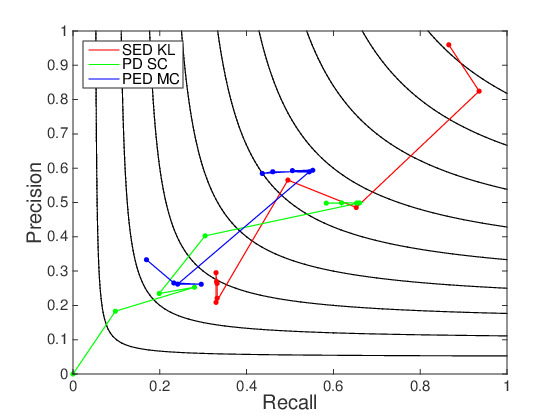
\includegraphics[width=0.47\linewidth] {evaluation/bonn_chairs/avg/avg_rec_prec}
   \label{fig:bonn_chairs_plot_avg_stat_a}
}
\subfigure[Cluster Count / F1 Score Plot]{
   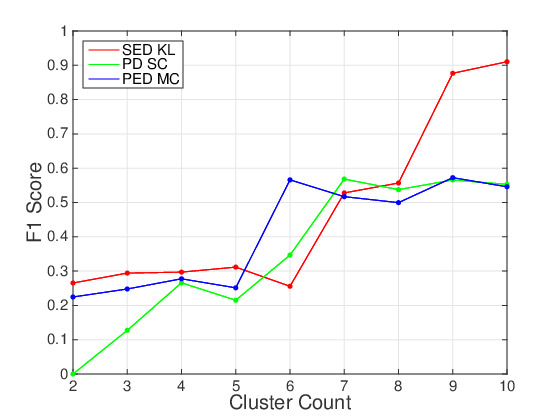
\includegraphics[width=0.47\linewidth] {evaluation/bonn_chairs/avg/avg_clusters_f1}
   \label{fig:bonn_chairs_plot_avg_stat_b}
}
\end{center}
\caption[Chair 3 Cast avg statistic plots]{Plots of the average performance of the four methods PED SC, PD MC, PED SC and PED MC for a varying number of clusters. The left plots shows the recall/precision plot and the figure on the right shows the F1 score alongside the number of clusters.}
\label{fig:bonn_chairs_plot_avg_stat}
\end{figure}

% TODO: update results according to the new mask:
% particularly, mention the following observations:
% ldof flow perform poor, since they are not able to successfully segment the lower chair part. this might be due to many reasons:
% on one hand, trajectories have to be relatively robust similar to each other to prevent oversegmentation potentially resulting from rotational movements. On the other hand, the movement of the lower chair segment strongly correlates with the upper (seat, lean) segment. Moreover, trajectories within this lower chair region are not very accurate due to shadows and lightning conditions.
% TODO: compare impact of results when using a complete chair mask
% TODO: compare results when using SRSF flows


\subsection{Influence of $\lambda$ on P-Affinities}
%START EXPERIMENT SETUP
chairs dataset, has no depth fields
use only LDOF flows and PD affinities
vary segmentation technique: SC, MC, KL

since we only use PD affinities, examine the influence of
$\lambda$ used to compute the affinity values and how it affects the quality of the segments, when running SC.
% END EXPERIMENT SETUP

\begin{table}[H]
\centering
\begin{tabular}{|l|l|r|l|l|}
\hline
\multicolumn{5}{|c|}{Comparission cars dataset 3 clusters}                        \\ \hline
              & \textbf{Density} & \textbf{Precision} & \textbf{Recall} & \textbf{F1 Score} \\ \hline
LDOF PD SC & 0.66829 & 91.0669 \%   & 92.8458 \%     & 91.9478 \%  \\ \hline
LDOF PD MC & 0.66829 & 91.0502 \%   & 88.9107 \%     & 89.9677 \%  \\ \hline              
LDOF SD & 0.69987 & 79.2541 \%   & 92.709 \%     & 85.4551 \%  \\ \hline
\end{tabular}
\caption[Cars Dataset]{My caption}
\label{tab:cars_ldof_quality}
\end{table}

\begin{figure}[H]
\begin{center}

\subfigure[GT]{
   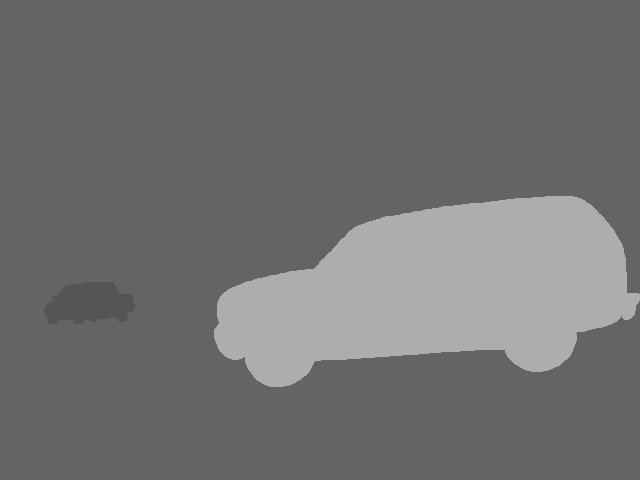
\includegraphics[width=0.48\linewidth] {evaluation/method_2d_ds/gt_1}
   \label{fig:cars_a}
}
\subfigure[LDOF PD SC]{
   \includegraphics[width=0.48\linewidth] {evaluation/method_2d_ds/ldof_pd_sc}
   \label{fig:cars_b}
}
~
\subfigure[LDOF PD MC]{
   \includegraphics[width=0.48\linewidth] {evaluation/method_2d_ds/ldof_pd_mc}
   \label{fig:cars_c}
}
\subfigure[LDOF SD]{
   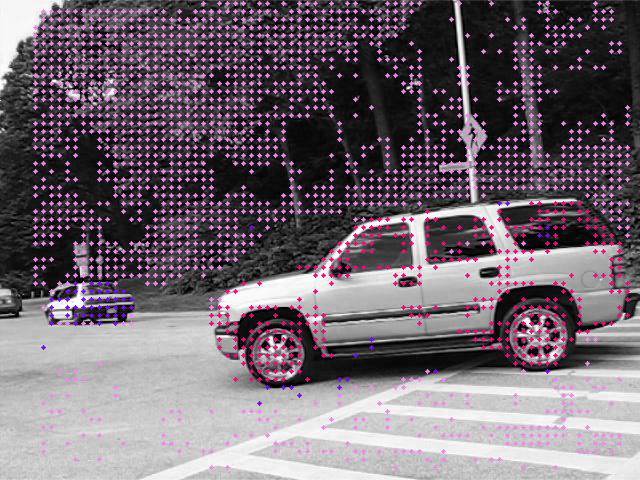
\includegraphics[width=0.48\linewidth] {evaluation/method_2d_ds/ldof_sd}
   \label{fig:cars_d}   
}
\end{center}
\caption[Method Comparison]{Visualization of segmentation resulting when running our pipeline on a dataset without depth information.}
\label{fig:cars_dataset}
\end{figure}




%dsf


\begin{table}[H]
\centering
\begin{tabular}{|c|c|c|c|c|}
\hline
\multicolumn{5}{|c|}{Performance Varying $\lambda$}                        \\ \hline
$\lambda$              & \textbf{Density} & \textbf{Precision} & \textbf{Recall} & \textbf{F1 Score} \\ \hline
5 & 0.59 & 99.70\%   & 57.99\%     & 73.33\%  \\ \hline
0.01 & 0.67 & 91.07\%   & 92.85\%     & 91.95\%  \\ \hline              
0.0001 & 0.67 & 47.91\%   & 49.62\%     & 48.75\%  \\ \hline
\end{tabular}
\caption[Cars Varying $\lambda$]{My caption}
\label{tab:cars_varying_lambas}
\end{table}

observations:
too large lambda values lead to not-fully covered segments
whereas choosing a too small lambda value leads to an oversegmentation.


\subsection{Evaluating Pipeline Modes}
%START EXPERIMENT SETUP
watercan dataset
run every possible flow-, affinity-,segmentation method pipeline combinations and evaluate their results on the available ground truth frames.
additionally, have a closer look at LRGBD flows and describe them qualitatively using this dataset.
% END EXPERIMENT SETUP

\begin{figure}[H]
\begin{center}
\subfigure[Frame 4]{
   \includegraphics[width=0.48\linewidth] {evaluation/watercan/ds/4}
   \label{fig:bonn_watercan_ds_a}
}
\subfigure[Ground Truth Frame 4]{
   \includegraphics[width=0.48\linewidth] {evaluation/watercan/gt/4}
   \label{fig:bonn_watercan_ds_b}
}
~
\subfigure[Frame 30]{
   \includegraphics[width=0.48\linewidth] {evaluation/watercan/ds/30}
   \label{fig:bonn_watercan_ds_c}
}
\subfigure[Ground Truth Frame 30]{
   \includegraphics[width=0.48\linewidth] {evaluation/watercan/gt/30}
   \label{fig:bonn_watercan_ds_d}
}
~
\subfigure[Frame 54]{
   \includegraphics[width=0.48\linewidth] {evaluation/watercan/ds/54}
   \label{fig:bonn_watercan_ds_e}
}
\subfigure[Ground Truth Frame 54]{
   \includegraphics[width=0.48\linewidth] {evaluation/watercan/gt/54}
   \label{fig:bonn_watercan_ds_f}
}
\end{center}
\caption[The Bonn Watercan Dataset]{Listing the Bonn Watercan Dataset and its ground truth frames.}
\label{fig:bonn_watercan_ds}
\end{figure}

\begin{figure}[H]
\begin{center}
\subfigure[LDOF PED SC]{
   \includegraphics[width=0.48\linewidth] {evaluation/meth_cmp_bonn_wc/ldof_ped_sc}
   \label{fig:bonn_wc_a}
}
\subfigure[LDOF PED MC]{
   \includegraphics[width=0.48\linewidth] {evaluation/meth_cmp_bonn_wc/ldof_ped_mc}
   \label{fig:bonn_wc_b}
}
~
\subfigure[SRSF PED SC]{
   \includegraphics[width=0.48\linewidth] {evaluation/meth_cmp_bonn_wc/srsf_ped_sc}
   \label{fig:bonn_wc_c}
}
\subfigure[SRSF PED MC]{
   \includegraphics[width=0.48\linewidth] {evaluation/meth_cmp_bonn_wc/srsf_ped_mc}
   \label{fig:bonn_wc_d}   
}
\end{center}
\caption[Method Comparison]{Visualization of merged segmentations when comparing various methods}
\label{fig:bonn_watercan_method_cmp}
\end{figure}

\begin{figure}[H]
\begin{center}
\subfigure[LDOF PD SC]{
   \includegraphics[width=0.48\linewidth] {evaluation/meth_cmp_bonn_wc/ldof_pd_sc}
   \label{fig:bonn_wc_ed}
}
\subfigure[LDOF PD MC]{
   \includegraphics[width=0.48\linewidth] {evaluation/meth_cmp_bonn_wc/ldof_pd_mc}
   \label{fig:bonn_wc_f}   
}
\end{center}
\caption[Method Comparison 2]{Visualization of merged segmentations when comparing various methods}
\label{fig:bonn_watercan_method_cmp_2}
\end{figure}


\begin{table}[]
\centering
\begin{tabular}{|l|r|l|l|}
\hline
\multicolumn{4}{|c|}{Method Comparison, 12 fixed Clusters, Bonn Watercan}                        \\ \hline
              & \textbf{Precision} & \textbf{Recall} & \textbf{F1 Score} \\ \hline
HS PD SC  & 80.00\%   & 31.26\%     & 44.95\%  \\ \hline
HS PD MC  & 41.98\%   & 39.38\%     & 40.64\%  \\ \hline              
HS PED SC  & 71.59\%   & 71.96\%     & 71.77\%  \\ \hline
HS PED MC  & 71.84\%   & 72.59\%     & 72.21\%  \\ \hline            
LDOF PD SC  & 72.78\%   & 66.19\%     & 69.33\%  \\ \hline
LDOF PD MC  & 34.17\%   & 45.67\%     & 39.09\%  \\ \hline              
LDOF PED SC  & 94.30\%   & 58.20\%     & 71.98\%  \\ \hline
LDOF PED MC  & 67.50\%   & 81.06\%     & 73.66\%  \\ \hline
SRSF PD SC & 96.25 \%   & 83.03\%     & 89.15\%  \\ \hline
SRSF PD MC & 95.12 \%   & 86.96\%     & 90.86\%  \\ \hline
SRSF PED SC & 90.00 \%   & 96.25\%     & 93.02\%  \\ \hline
SRSF PED MC & 94.23 \%   & 95.04\%     & 94.63\%  \\ \hline
LRGBD PD SC & 0 \%   & 0 \%     & 0 \%  \\ \hline
LRGBD PD MC & 0 \%   & 0 \%     & 0 \%  \\ \hline
LRGBD PED SC & 30.00\%   & 16.68\%     & 21.43\%  \\ \hline
LRGBD PED MC & 31.23\%   & 16.32\%     & 21.44\%  \\ \hline
\end{tabular}
\caption[Method Comparission Bonn Watercan]{My caption}
\label{tab:bonn_wc_methods}
\end{table}


observations
SRSF outperforms every other flow method
using depth maps leads too a drastically improves the segmentation quality.
HS with depth cues almost achieves the same segmentation performance as when using LDOF flows. However, keep in mind that HS flows are computed about roughly 20 times faster than LDOF flows.
even though the LRGBD flows are supposed to be competitive against SRSF flows, using them yields a poor segmentation. This is due the fact, that LRGBD flows are estimated by segmenting the flows with respect to their depth layers.


\begin{figure}[H]
\begin{center}

\subfigure[Extracted Layers Frame 30]{
   \includegraphics[width=0.31\linewidth] {evaluation/lrgbd_issues/layers_30}
   \label{fig:issues_lrgbd_flows_a}
}
\subfigure[Forward Flow Frame 30]{
   \includegraphics[width=0.31\linewidth] {evaluation/lrgbd_issues/fw_flow_30}
   \label{fig:issues_lrgbd_flows_b}
}
\subfigure[Segmentation PED MC Frame 30]{
   \includegraphics[width=0.31\linewidth] {evaluation/lrgbd_issues/seg_30}
   \label{fig:issues_lrgbd_flows_c}
}
\end{center}
\caption[Issue with LRGBD Flows]{foobar}
\label{fig:issues_lrgbd_flows}
\end{figure}

observations:
LRGBD flows yield a poor segmentation when used by our pipeline.
having a closer look at the generated flow fields, we observe, that the flow fields are locally homogenous within the layer they belongs to / are intersecting.
the resulting segmentation when using lrgbd flows separates the layers rather than moving objects.



\subsection{Varying Cluster Count on SC and MC}
% START EXPERIMENT DESC
use LDOF flows and run the pipeline modes: PD SC, PD MC, PED SC, PED MC
vary the number of clusters and evaluate the resulting segmentations
This experiment should examine 
This experiment should examine the behaviour of these modes using an increasing number of clusters.

% END EXPERIMENT DESC


%TODO: add figure showing segmentation of worst performance: worst/best

\begin{figure}[H]
\begin{center}
\subfigure[Frame 30]{
   \includegraphics[width=0.31\linewidth] {evaluation/chairs_3_cast/ds/30}
   \label{fig:chair_3_cast_dataset_a}
}
\subfigure[Frame 45]{
   \includegraphics[width=0.31\linewidth] {evaluation/chairs_3_cast/ds/45}
   \label{fig:chair_3_cast_dataset_b}
}
\subfigure[Frame 60]{
   \includegraphics[width=0.31\linewidth] {evaluation/chairs_3_cast/ds/60}
   \label{fig:chair_3_cast_dataset_c}
}
\end{center}
\caption[Chair 3 Cast Dataset]{Listing of 4 ascending frames of the our Chair 3 Cast dataset.}
\label{fig:chair_3_cast_dataset}
\end{figure}

\begin{figure}[H]
\begin{center}

\subfigure[Gt Frame 45]{
   \includegraphics[width=0.31\linewidth] {evaluation/chairs_3_cast/gt/45}
   \label{fig:chair_3_cast_masks_a}
}
\subfigure[GT Frame 60]{
   \includegraphics[width=0.31\linewidth] {evaluation/chairs_3_cast/gt/60_amb}
   \label{fig:chair_3_cast_masks_b}
}
\subfigure[GT Frame 75]{
   \includegraphics[width=0.31\linewidth] {evaluation/chairs_3_cast/gt/75_amb}
   \label{fig:chair_3_cast_masks_c}
}
\end{center}
\caption[Chair 3 Cast Masks]{An illustration of the ground truth masks we use to evaluate the performance of our segmentations.}
\label{fig:chair_3_cast_masks}
\end{figure}

\begin{figure}[H]
\begin{center}

\subfigure[5 Clusters PED MC]{
   \includegraphics[width=0.47\linewidth] {evaluation/chairs_3_cast/best/ped_mc_c_5}
   \label{fig:chair_3_cast_masks_a}
}
\subfigure[10 Clusters PED MC]{
   \includegraphics[width=0.47\linewidth] {evaluation/chairs_3_cast/best/ped_mc_c_10}
   \label{fig:chair_3_cast_masks_b}
}
~
\subfigure[15 Clusters PD SC]{
   \includegraphics[width=0.47\linewidth] {evaluation/chairs_3_cast/best/pd_sc_c_15}
   \label{fig:chair_3_cast_masks_c}
}
\subfigure[20 Clusters PD SC]{
   \includegraphics[width=0.47\linewidth] {evaluation/chairs_3_cast/best/ped_mc_c_20}
   \label{fig:chair_3_cast_masks_d}
}
\end{center}
\caption[Chair 3 Cast Winner]{Listing the four top segmentation results of frame 60 based on the scored F1 value.}
\label{fig:chair_3_cast_best_f_score_results}
\end{figure}

%
\begin{figure}[H]
\begin{center}

\subfigure[5 Clusters PED MC]{
   \includegraphics[width=0.47\linewidth] {evaluation/chairs_3_cast/merged/ped_mc_c_5}
   \label{fig:chair_3_cast_masks_merged_a}
}
\subfigure[10 Clusters PED MC]{
   \includegraphics[width=0.47\linewidth] {evaluation/chairs_3_cast/merged/ped_mc_c_10}
   \label{fig:chair_3_cast_masks_merged_b}
}
~
\subfigure[15 Clusters PD SC]{
   \includegraphics[width=0.47\linewidth] {evaluation/chairs_3_cast/merged/pd_sc_c_15}
   \label{fig:chair_3_cast_masks_merged_c}
}
\subfigure[20 Clusters PED MC]{
   \includegraphics[width=0.47\linewidth] {evaluation/chairs_3_cast/merged/ped_mc_c_20}
   \label{fig:chair_3_cast_masks_merged_d}
}
\end{center}
\caption[Chair 3 Cast Winner]{Visualization of the merged segmentations of the figures shown in figure $\ref{fig:chair_3_cast_best_f_score_results}$.}
\label{fig:chair_3_cast_best_f_score_results_merged}
\end{figure}

\begin{table}[H]
\centering
\begin{tabular}{|l|c|c|c|c|}
\hline
\multicolumn{5}{|c|}{Average Precision} \\ \hline
\textbf{Method / \#Cluster} & 5 & 10 & 15 & 20 \\ \hline
PD SC & 18.01\% & \textbf{55.17}\% & \textbf{55.12}\% & \textbf{56.23}\% \\ \hline
PD MC & \textbf{38.70}\% & 38.14\% & 45.65\% & 49.64\% \\ \hline
PED SC & 13.14\% & 35.29\% & 50.75\% & 52.14\%  \\ \hline
PED MC & 26.81\% & 42.94\% & 38.70\% & \textbf{56.23}\% \\ \hline
\multicolumn{5}{|c|}{Average Recall} \\ \hline
PD SC & 12.34\% & 19.22\% & 38.13\% & 47.82\% \\ \hline
PD MC & 13.10\% & 24.51\% & \textbf{44.07}\% & \textbf{53.50}\% \\ \hline
PED SC & 10.20\% & 28.29\% & 39.24\% & 33.75\% \\ \hline
PED MC & \textbf{19.37}\% & \textbf{38.86}\% & 41.88\% & 50.07\% \\ \hline
\multicolumn{5}{|c|}{Average F1 Score} \\ \hline
PD SC & 14.02\% & 28.47\% & \textbf{45.04}\% & 51.59\% \\ \hline
PD MC & 19.50\% & 29.79\% & 44.63\% & 51.40\% \\ \hline
PED SC & 11.48\% & 30.89\% & 43.88\% & 40.69\% \\ \hline
PED MC & \textbf{21.97}\% & \textbf{40.63}\% & 40.12\% & \textbf{52.58}\% \\ \hline
\end{tabular}
\caption[Chair 3 Cast: Average Precision Scores]{Average performance on the chair 3 cast dataset for a varying number of clusters. For large and low cluster counts, PED MC achieves the best F1 scores.}
\label{tab:chair_3_cast_avg_performance}
\end{table}

\begin{figure}[H]
\begin{center}

\subfigure[Recall / Precision Plot]{
   \includegraphics[width=0.47\linewidth] {evaluation/chairs_3_cast/avg/avg_prec_rec}
   \label{fig:chair_3_cast_plot_avg_stat_a}
}
\subfigure[Cluster Count / F1 Score Plot]{
   \includegraphics[width=0.47\linewidth] {evaluation/chairs_3_cast/avg/avg_clust_f1}
   \label{fig:chair_3_cast_plot_avg_stat_b}
}
\end{center}
\caption[Chair 3 Cast avg statistic plots]{Plots of the average performance of the four methods PED SC, PD MC, PED SC and PED MC for a varying number of clusters. The left plots shows the recall/precision plot and the figure on the right shows the F1 score alongside the number of clusters.}
\label{fig:chair_3_cast_plot_avg_stat}
\end{figure}

\begin{figure}[H]
\begin{center}
\subfigure[Ground truth frame 60]{
   \includegraphics[width=0.31\linewidth] {evaluation/chairs_3_cast/worst_best/60_amb}
   \label{fig:chair_3_cast_gt_worst_best_a}
}
\subfigure[Worst F1 Score Frame 60]{
   \includegraphics[width=0.31\linewidth] {evaluation/chairs_3_cast/worst_best/ped_sc_c_5_f_60}
   \label{fig:chair_3_cast_gt_worst_best_b}
}
\subfigure[Best F1 Score Frame 60]{
   \includegraphics[width=0.31\linewidth] {evaluation/chairs_3_cast/worst_best/ped_mc_c_20_f_60}
   \label{fig:chair_3_cast_gt_worst_best_c}
}
\end{center}
\caption[Chair 3 Cast Worst/Best Result]{Comparison of the worst- (center) and the best (right) segmentation results according to the F1 measure using the shown mask on the left.}
\label{fig:chair_3_cast_gt_worst_best}
\end{figure}


c 5
density:0.7114
density:0.7114
density:0.6062
density:0.6062

c 10
density: 0.7114
density:0.7114
density:0.6062
density:0.6062

c 15
density:0.71138
density:0.7114
density:0.6062
density:0.6062


avgs

%c20
%pd sc density: 0.72198\%
%pd mc density:0.71138\%
%ped sc density:0.6062\%
%ped mc density:0.6062\%


% TODO: cereal SRSF PED MC, LDOF PED MC
%TODO: mache evaluation über alle datasets

% TODO wh1	: PED SC PED MC
% matrix clusters/eigenvectors for MC
% c = 2, 3, 4, 5
% eigs 2 3 4 5

% TODO artificial results

% rotating statue

\subsection{Dependence of Eigenvector-Cluster Count on MC}
In this experiment, we use the \textbf{WH} dataset and again only use LDOF flows. An example frame with its ground truth image is shown in figure $\ref{fig:wh1_dataset}$.
\begin{figure}[H]
\begin{center}
\subfigure[Frame 40]{
   \includegraphics[width=0.47\linewidth] {evaluation/wh1/40}
   \label{fig:wh1_performance_a}
}
\subfigure[GT]{
   \includegraphics[width=0.47\linewidth] {evaluation/wh1/gt/40}
   \label{fig:wh1_performance_b}
}
\end{center}
\caption[Segmentations Waving Hand]{foobar}
\label{fig:wh1_dataset}
\end{figure}
Initially, run the pipeline modes: PD SC, PD MC, PED SC, PED MC. \\ \\
Afterwards, run the mode PED MC once again for a varying number of used eigenvectors-clusters. \\ \\
Since the MC both parameters determine the final quality of this method, this should us give a better understanding of this parameters. How does the result change when we fix the cluster count but vary the number of eigenvectors or how does the segmentation quality improve for a fixed number of eigenvectors, when varying the total number of used clusters. Hence, a set of eigenvector-,cluster-count combinations are run their segmentations are evaluated using the available GT images. \\ \\
This should give us a better understanding of the behaviour of the MC method and the influence of those parameter values. \\ \\

In this first sub-experiment we generate the segmentations running the pipeline modes: PD SC, PD MC, PED SC, PED MC. We fix the number of clusters and eigenvectors and set them equals six. Some segmentations are shown in figure $\ref{fig:wh1_performance}$.
\begin{figure}[H]
\begin{center}
\subfigure[PD SC]{
   \includegraphics[width=0.47\linewidth] {evaluation/wh1/segmentations/ldof_pd_sc}
   \label{fig:wh1_performance_a}
}
\subfigure[PD MC]{
   \includegraphics[width=0.47\linewidth] {evaluation/wh1/segmentations/ldof_pd_mc}
   \label{fig:wh1_performance_b}
}
\subfigure[PED SC]{
   \includegraphics[width=0.47\linewidth] {evaluation/wh1/segmentations/ldof_ped_sc}
   \label{fig:wh1_performance_c}
}
\subfigure[PED MC]{
   \includegraphics[width=0.47\linewidth] {evaluation/wh1/segmentations/ldof_ped_mc}
   \label{fig:wh1_performance_d}
}
\end{center}
\caption[Segmentations Waving Hand]{foobar}
\label{fig:wh1_performance}
\end{figure}
The corresponding statistics of those segmentations are listed in table $\ref{tab:wh1_performance}$.
\begin{table}[H]
\centering
\begin{tabular}{|c|c|c|c|}
\hline
\multicolumn{4}{|c|}{Performance Waving Hand dataset}                        \\ \hline
Method & \textbf{Precision} & \textbf{Recall} & \textbf{F1 Score} \\ \hline
PD SC & 69.67\%   & 58.66\%     & 63.69\%  \\ \hline
PD MC & 55.16\%   & 68.076\%     & 60.94\%  \\ \hline
PED SC & 75.40\%   & 62.90\%     & 68.58\%  \\ \hline
PED MC & 71.47\%   & 67.39\%     & 69.37\%  \\ \hline               
\end{tabular}
\caption[Cars Varying $\lambda$]{My caption}
\label{tab:wh1_performance}
\end{table}
We observe that:
PED MC achieves a better results than the other methods.
Additionally, using depths seems to increase the quality of the segmentations. \\ \\
Next, we perform sub-experiment two. In this we examine the bahaviour of PED MC method for a varying the eigenvalue-cluster count. Additionally, we want to investigate the dependence between these two parameter to better understand them. \\ \\
For 2..6 clusters for 2..6 eigenvectors plot results to demonstrate influence
of number of clusters,eigenvectors. The corresponding statistics are listed in table $\ref{tab:wh_ev_c}$. To give the reader a easier way to understand the results we visualized the resulting statistics. For fixed cluster counts, we plotted the recall-precession and the eigenvector-f1 score graphs. Moreover, for fixed eigenvector counts we plotted the resulting recall-precession and clusters-f1 score graphs. The graphs are given in figure $\ref{fig:wh1_performance_var_ev_c_graphs}$.
\begin{figure}[H]
\begin{center}
\subfigure[Varying Clusters Recall/Precision Plot]{
   \includegraphics[width=0.47\linewidth] {evaluation/wh1/perf_ev_c/clusters_rec_prec}
   \label{fig:wh1_performance_var_ev_a}
}
\subfigure[Varying Clusters EV/F1 Score Plot]{
   \includegraphics[width=0.47\linewidth] {evaluation/wh1/perf_ev_c/clusters_ev_f1}
   \label{fig:wh1_performance_var_ev_b}
}
\subfigure[Varying EV Recall/Precision Plot]{
   \includegraphics[width=0.47\linewidth] {evaluation/wh1/perf_ev_c/ev_rec_prec}
   \label{fig:wh1_performance_var_ev_c}
}
\subfigure[Varying EV Clusters/F1 Score Plot]{
   \includegraphics[width=0.47\linewidth] {evaluation/wh1/perf_ev_c/ev_c_f1}
   \label{fig:wh1_performance_var_ev_d}
}
\end{center}
\caption[Plot Performance Varying CLuster/Eigenvectors]{foobar}
\label{fig:wh1_performance_var_ev_c_graphs}
\end{figure}
% TODO: state observations here: 
\begin{table}[H]
\centering
\begin{tabular}{|l|c|c|c|c|c|}
\hline
\multicolumn{6}{|c|}{Performance Varying Eigenvectors/Clusters PED MC} \\ \hline
\multicolumn{6}{|c|}{Precision} \\ \hline
\textbf{Eigenvectors / Clusters} & 2 & 3 & 4 & 5 & 6 \\ \hline
2 & 7.03\% & 29.28\% & 33.80\% & 59.61\% & 48.63\%  \\ \hline
3 & 6.95\% & 28.62\% & 40.45\% & 57.17\% & 45.59\%  \\ \hline
4 & 6.99\% & 30.28\% & 46.90\% & 43.53\% & 65.60\%  \\ \hline
5 & 7.05\% & 30.28\% & 49.35\% & 53.55\% & 70.23\%  \\ \hline
6 & 7.05\% & 30.28\% & 50.11\% & 53.81\% & 71.47\%  \\ \hline
\multicolumn{6}{|c|}{Recall} \\ \hline
2 & 23.64\% & 40.45\% & 36.28\% & 79.73\% & 50.27\%  \\ \hline
3 & 23.64\% & 41.17\% & 40.45\% & 57.17\% & 61.04\%  \\ \hline
4 & 23.64\% & 41.17\% & 57.20\% & 60.50\% & 79.28\%  \\ \hline
5 & 24.09\% & 41.17\% & 52.55\% & 54.29\% & 71.71\%  \\ \hline
6 & 24.09\% & 41.17\% & 52.55\% & 53.42\% & 67.39\%  \\ \hline
\multicolumn{6}{|c|}{F1 Score} \\ \hline
2 & 10.83\% & 33.97\% & 35.00\% & 68.22\% & 49.43\%  \\ \hline
3 & 10.74\% & 33.77\% & 32.97\% & 50.94\% & 52.20\%  \\ \hline
4 & 10.79\% & 34.90\% & 51.54\% & 50.63\% & 71.79\%  \\ \hline
5 & 10.91\% & 34.90\% & 50.90\% & 53.92\% & 70.97\%  \\ \hline
6 & 10.91\% & 34.90\% & 51.30\% & 53.62\% & 69.37\%  \\ \hline
\end{tabular}
\caption[Performance Varying Eigenvector-Cluster]{My caption}
\label{tab:wh_ev_c}
\end{table}

\subsection{Quality Product Affinities}

\begin{figure}[H]
\begin{center}
\subfigure[Frame 15]{
   \includegraphics[width=0.47\linewidth] {evaluation/two_chairs/ds/15}
   \label{fig:two_chairs_dataset_a}
}
\subfigure[Frame 40]{
   \includegraphics[width=0.47\linewidth] {evaluation/two_chairs/ds/40}
   \label{fig:two_chairs_dataset_b}
}
~
\subfigure[GT 15]{
   \includegraphics[width=0.47\linewidth] {evaluation/two_chairs/gt/15}
   \label{fig:two_chairs_dataset_c}
}
\subfigure[GT 40]{
   \includegraphics[width=0.47\linewidth] {evaluation/two_chairs/gt/40}
   \label{fig:two_chairs_dataset_d}
}
\end{center}
\caption[Two Chairs Dataset]{foobar}
\label{fig:two_chairs_dataset}
\end{figure}

\begin{figure}[H]
\begin{center}
\subfigure[PD SC Frame 15]{
   \includegraphics[width=0.22\linewidth] {evaluation/two_chairs/segmentations/15/pd_sc}
   \label{fig:two_chairs_seg_f_15_a}
}
\subfigure[PD MC Frame 15]{
   \includegraphics[width=0.22\linewidth] {evaluation/two_chairs/segmentations/15/pd_mc}
   \label{fig:two_chairs_seg_f_15_b}
}
\subfigure[PED SC Frame 15]{
   \includegraphics[width=0.22\linewidth] {evaluation/two_chairs/segmentations/15/ped_sc}
   \label{fig:two_chairs_seg_f_15_c}
}
\subfigure[PED MC Frame 15]{
   \includegraphics[width=0.22\linewidth] {evaluation/two_chairs/segmentations/15/ped_mc}
   \label{fig:two_chairs_seg_f_15_d}
}
~
\subfigure[PD SC Frame 40]{
   \includegraphics[width=0.22\linewidth] {evaluation/two_chairs/segmentations/40/pd_sc}
   \label{fig:two_chairs_seg_f_15_e}
}
\subfigure[PD MC Frame 40]{
   \includegraphics[width=0.22\linewidth] {evaluation/two_chairs/segmentations/40/pd_mc}
   \label{fig:two_chairs_seg_f_15_f}
}
\subfigure[PED SC Frame 40]{
   \includegraphics[width=0.22\linewidth] {evaluation/two_chairs/segmentations/40/ped_sc}
   \label{fig:two_chairs_seg_f_15_g}
}
\subfigure[PED MC Frame 40]{
   \includegraphics[width=0.22\linewidth] {evaluation/two_chairs/segmentations/40/ped_mc}
   \label{fig:two_chairs_seg_f_15_h}
}
\end{center}
\caption[Two Chairs Segmentation]{foobar}
\label{fig:two_chairs_seg_f_15_40}
\end{figure}

\begin{table}[H]
\centering
\begin{tabular}{|c|c|c|c|}
\hline
\multicolumn{4}{|c|}{Performance Two Chairs dataset}                        \\ \hline
Method & \textbf{Precision} & \textbf{Recall} & \textbf{F1 Score} \\ \hline
PD SC & 88.1991\%   & 65.3383\%     & 74.9641\%  \\ \hline
PD MC & 87.9687\%   & 60.0087\%     & 65.3910\%  \\ \hline 
PED SC & 97.1673\%   & 73.2142\%     & 76.4836\%  \\ \hline
PED MC & 96.0427\%   & 96.8572\%     & 96.4160\%  \\ \hline               
\end{tabular}
\caption[Cars Varying $\lambda$]{My caption}
\label{tab:two_chairs_performance}
\end{table}



\begin{figure}[H]
\begin{center}
\subfigure[1 Iteration]{
   \includegraphics[width=0.47\linewidth] {evaluation/two_chairs/iters/iter_1}
   \label{fig:two:chairs_segmentations_ped_mc_iters_a}
}
\subfigure[2 Iterations]{
   \includegraphics[width=0.47\linewidth] {evaluation/two_chairs/iters/iter_2}
   \label{fig:two:chairs_segmentations_ped_mc_iters_b}
}
~
\subfigure[3 Iterations]{
   \includegraphics[width=0.47\linewidth] {evaluation/two_chairs/iters/iter_3}
   \label{fig:two:chairs_segmentations_ped_mc_iters_b}
}
\subfigure[5 Iterations]{
   \includegraphics[width=0.47\linewidth] {evaluation/two_chairs/iters/iter_5}
   \label{fig:two:chairs_segmentations_ped_mc_iters_b}
}
\end{center}
\caption[Segmentations Waving Hand]{foobar}
\label{fig:two:chairs_segmentations_ped_mc_iters}
\end{figure}


%
\begin{figure}[H]
\begin{center}
\subfigure[Recall/Precision Plot]{
   \includegraphics[width=0.47\linewidth] {evaluation/two_chairs/performance_iter/rec_prec}
   \label{fig:two_chairs_ped_mc_iterations_a}
}
\subfigure[Iterations/F1 Score Plot]{
   \includegraphics[width=0.47\linewidth] {evaluation/two_chairs/performance_iter/iter_f1}
   \label{fig:two_chairs_ped_mc_iterations_b}
}
\end{center}
\caption[Convergence PED MC]{foobar}
\label{fig:two_chairs_ped_mc_iterations}
\end{figure}


\begin{table}[H]
\centering
\begin{tabular}{|c|c|c|c|}
\hline
\multicolumn{4}{|c|}{Convergence PED MC Two Chairs}                        \\ \hline
Iteration & \textbf{Precision} & \textbf{Recall} & \textbf{F1 Score} \\ \hline
0 & 0\%   & 0\%     & 0\%  \\ \hline
1 & 83.55\%   & 95.97\%     & 89.33\%  \\ \hline
2 & 92.24\%   & 93.28\%     & 92.76\%  \\ \hline 
3 & 96.89\%   & 94.42\%     & 95.64\%  \\ \hline
4 & 97.14\%   & 94.49\%     & 95.80\%  \\ \hline
5 & 97.22\%   & 94.51\%     & 95.84\%  \\ \hline               
\end{tabular}
\caption[Convergence PED MC]{My caption}
\label{tab:two_chairs_ped_mc_iterations}
\end{table}

\subsection{Quality of LDOF P-Affnities}
particular hard dataset, long frame sequence, very shaky camera, strong shadows, deformation due to human hand.
ev,c
20,15
ldof

\begin{figure}[H]
\begin{center}
\subfigure[Frame 40]{
   \includegraphics[width=0.47\linewidth] {evaluation/bonn_cerealbox/ds/f_40}
   \label{fig:bonn_cerealbox_ds_a}
}
\subfigure[GT Frame 40]{
   \includegraphics[width=0.47\linewidth] {evaluation/bonn_cerealbox/ds/gt_40}
   \label{fig:bonn_cerealbox_ds_b}
}
\end{center}
\caption[Bonn Cerealbox Dataset]{foobar}
\label{fig:bonn_cerealbox_ds}
\end{figure}

\begin{figure}[H]
\begin{center}
\subfigure[PD MC]{
   \includegraphics[width=0.47\linewidth] {evaluation/bonn_cerealbox/segmentations/ldof_pd_mc}
   \label{fig:bonn_cerealbox_segmentations_mc_methods_a}
}
\subfigure[PED MC]{
   \includegraphics[width=0.47\linewidth] {evaluation/bonn_cerealbox/segmentations/ldof_ped_mc}
   \label{fig:bonn_cerealbox_segmentations_mc_methods_b}
}
\end{center}
\caption[Bonn Cerealbox Segmentations]{foobar}
\label{fig:bonn_cerealbox_segmentations_mc_methods}
\end{figure}


\begin{table}[H]
\centering
\begin{tabular}{|c|c|c|c|}
\hline
\multicolumn{4}{|c|}{Performance Bonn Cerealbox dataset}                        \\ \hline
Method & \textbf{Precision} & \textbf{Recall} & \textbf{F1 Score} \\ \hline
PD SC & 32.26\%   & 33.33\%     & 32.79\%  \\ \hline
PD MC & 73.81\%   & 80.57\%     & 77.04\%  \\ \hline 
PED SC & 76.15\%   & 86.69\%     & 81.08\%  \\ \hline
PED MC & 88.87\%   & 91.98\%     & 90.40\%  \\ \hline               
\end{tabular}
\caption[Cars Varying $\lambda$]{My caption}
\label{tab:bonn_cerealbox_performance}
\end{table}

\subsection{PED MC using different flows}
This experiment should examine how some of our methods perform when running a particular difficult dataset. For this purpose we use the statue statue. In particular it has the following difficulties:
\begin{itemize}
  \item movement, deformation (hands), rotation (spinning statue on rotator), removing parts.
  \item many invalid regions due to missing depth information
\end{itemize}
Some frames of this dataset, as well as their corresponding ground truth images are listed in figure $\ref{fig:statue_ds}$.
\begin{figure}[H]
\begin{center}
\subfigure[Frame 25]{
   \includegraphics[width=0.47\linewidth] {evaluation/statue/ds/30}
   \label{fig:statue_ds_a}
}
\subfigure[Frame 30]{
   \includegraphics[width=0.47\linewidth] {evaluation/statue/gt/30}
   \label{fig:statue_ds_b}
}
~
\subfigure[Frame 35]{
   \includegraphics[width=0.47\linewidth] {evaluation/statue/ds/60}
   \label{fig:statue_ds_c}
}
\subfigure[Frame 40]{
   \includegraphics[width=0.47\linewidth] {evaluation/statue/gt/60}
   \label{fig:statue_ds_d}
}
\end{center}
\caption[Statue Dataset]{foobar}
\label{fig:statue_ds}
\end{figure}
We only vary the used flow method and fix the pipeline mode to PED MC. In other words we run the following three modes: LDOF PED MC, SRSF PED MC, LGBDR PED MC. \\ \\
The achieved performances are listed in table $\ref{tab:statue_performance}$ and visual segmentations are depicted in figure $\ref{fix:alley_segmentations}$.
\begin{figure}[H]
\begin{center}
\subfigure[LDOF PED MC]{
   \includegraphics[width=0.31\linewidth] {evaluation/statue/segmentations/f30/ldof_ped_mc}
   \label{fix:alley_segmentations_a}
}
\subfigure[SRSF PED MC]{
   \includegraphics[width=0.31\linewidth] {evaluation/statue/segmentations/f30/srsf_ped_mc}
   \label{fix:alley_segmentations_b}
}
\subfigure[LGBDR PED MC]{
   \includegraphics[width=0.31\linewidth] {evaluation/statue/segmentations/f30/lrgbd_ped_mc}
   \label{fix:alley_segmentations_c}
}
~
\subfigure[LDOF PED MC]{
   \includegraphics[width=0.31\linewidth] {evaluation/statue/segmentations/f60/ldof_ped_mc}
   \label{fix:alley_segmentations_d}
}
\subfigure[SRSF PED MC]{
   \includegraphics[width=0.31\linewidth] {evaluation/statue/segmentations/f60/srsf_ped_mc}
   \label{fix:alley_segmentations_e}
}
\subfigure[LGBDR PED MC]{
   \includegraphics[width=0.31\linewidth] {evaluation/statue/segmentations/f60/lrgbd_ped_mc}
   \label{fix:alley_segmentations_f}
}
\end{center}
\caption[Bonn Cerealbox Segmentations]{foobar}
\label{fix:alley_segmentations}
\end{figure}

\begin{table}[H]
\centering
\begin{tabular}{|c|c|c|c|}
\hline
\multicolumn{4}{|c|}{Performance Statue dataset}                        \\ \hline
Method & \textbf{Precision} & \textbf{Recall} & \textbf{F1 Score} \\ \hline
LDOF PED MC & 69.93\%   & 38.23\%     & 49.44\%  \\ \hline
SRSF PED MC & 72.47\%   & 70.68\%     & 71.56\%  \\ \hline
LRGBD PED MC & 61.46\%   & 8.37\%     & 14.73\%  \\ \hline              
\end{tabular}
\caption[Performance Statue]{My caption}
\label{tab:statue_performance}
\end{table}

\subsection{Overall Performance}
evaluating the segmentation quality of some of our methods using five our datasets and three of their ground truth frames. We use LDOF and SRSF flows. \\ \\
In this last experiment we perform an overall evaluation of our main methods using their standard parameter setup. For this evaluation we use five datasets (Cerealbox, Chairs, Watercan, Waving-Arm, Statue). \\ \\
For generating motion segmentations we run a subset of the cross-combinations between the used flow methods, two-and tree d motions, and the segmentation method. In particular we want to compare the quality of the two pipeline methods LDOF PC SC and SRSF PED MC. The first mostly resembles Brox' original implementation, whereas the former corresponds to an adapted, enhanced version making use of depth cues, more robust flow fields and a reliable segmentation method. Moreover, we also run weaker versions of our enhanced version to demonstrate that by reducing one particular pipeline component, the overall segmentation suffers. Moreover, we also run a strong graph-partitioning algorithm called KL which yields a superior segmentation quality. Lastly, To have a better comparison we also run T. Brox' Graphcut method on our datasets and evaluate its quality. \\ \\
Each method computes the segmentation on every dataset. For each dataset we use three ground-truth images, which we use to evaluate the quality of the resulting segmentations. The averaged performance is listed in table \ref{tab:overall_performance}.

\begin{table}[H]
\centering
\begin{tabular}{|c|c|c|c|}
\hline
\multicolumn{4}{|c|}{Overall Performance}                        \\ \hline
Method & \textbf{Precision} & \textbf{Recall} & \textbf{F1 Score} \\ \hline
LDOF PD SC & 60.04\%   & 35.99\%     & 45.00\%  \\ \hline
LDOF PED MC & 59.30\%   & 64.79\%     & 61.93\%  \\ \hline
SRSF PED MC & \textbf{76.52}\%   & \textbf{83.47}\%     & \textbf{79.84}\%  \\ \hline
SRSF PED SC & 60.23\%   & 49.62\%     & 54.41\%  \\ \hline 
SRSF PD MC & 61.85\%   & 55.06\%     & 58.25\%  \\ \hline
SRSF SED KL & 87.19\%   & 91.77\%     & 89.42\%  \\ \hline
Brox's GraphCut & 30.88\%   & 25.34\%     & 27.84\%  \\ \hline                   
\end{tabular}
\caption[Overall Performance]{My caption}
\label{tab:overall_performance}
\end{table}
We observe the following facts: Methods using SRSF flows achieve better results than those using LDOF flows. Methods that make use of depth cues are generally performing better than two dimensional approaches. And lastly, using min cut for generating the segmentation is better than running spectral clustering. \\ \\
Additionally, Kernighan Lin yields the best segmentations among all segmentation methods. In fact is superior compared with the other methods. However, segmenting trajectories via KL takes a very long time (about 20 hours per 5000 Trajectories) and has in fact a runtime complexity number of trajectories to the power of three. Interestingly, Brox's GraphCut, using its standard parameter setup does not generate very good segmentation results. To be fair, however, we have to mention, that we use a competitive parameter setting dedicated for our pipeline and also, GraphCut does not make use of depth cues (which seems a key ingredient to increase the segmentation quality).




